\documentclass{ieeeaccess}
\usepackage{cite}
\usepackage{amsmath,amssymb,amsfonts}
\usepackage{algorithm}
\usepackage{algorithmicx}
\usepackage{algpseudocode}
%% \usepackage{caption}
\usepackage{graphicx}
\usepackage{textcomp}

\usepackage{bm}

\usepackage{multirow}

\usepackage{url}

\usepackage{array}
\setlength\extrarowheight{3pt}


\algnewcommand\algorithmicforeach{\textbf{for each}}
\algdef{S}[FOR]{ForEach}[1]{\algorithmicforeach\ #1\ \algorithmicdo}

\providecommand{\e}[1]{\ensuremath{\times 10^{#1}}}

\def\BibTeX{{\rm B\kern-.05em{\sc i\kern-.025em b}\kern-.08em
    T\kern-.1667em\lower.7ex\hbox{E}\kern-.125emX}}

\begin{document}
\history{Date of publication xxxx 00, 0000, date of current version xxxx 00, 0000.}
\doi{10.1109/ACCESS.2017.DOI}

\title{Using Fuzzy Inference Systems for the Creation of Forex Market Predictive Models}
\author{
    \uppercase{Amaury Hernandez-\'{A}guila\authorrefmark{1},
    Mario Garc\'{i}a-Valdez\authorrefmark{1},
    Juan-Julián Merelo-Guerv\'{o}s\authorrefmark{2},
    Manuel Castañ\'{o}n-Puga\authorrefmark{3} and
    Oscar Castillo L\'{o}pez\authorrefmark{1}}}

\address[1]{National Technological Institute of Mexico, Calzada Del Tecnoló\'{o}ico s/n, Fraccionamiento Tomas Aquino, Tijuana, BC 22414 México (e-mail: {amerhag,mario,ocastillo}@tectijuana.edu.mx)}
\address[2]{University of Granada, Campus Aynadamar Daniel Saucedo Aranda s/n, Granada 18071, 80523 Spain (e-mail: jmerelo@geneura.ugr.es)}
\address[3]{Autonomous University of Baja California, Calzada Universidad 14418, Tijuana, BC, 22390, México (e-mail: puga@uabc.edu.mx)}
% Grant information.
% TODO 1:
\tfootnote{Space for acknowledgments.}

\markboth
{Hernandez-\'{A}guila \headeretal: Using Fuzzy Inference Systems... }
{Hernandez-\'{A}guila \headeretal: Using Fuzzy Inference Systems... }
% Do we need to change this?
% TODO 2: 

\corresp{Corresponding author: Mario Garc\'{i}a-Valdez (e-mail: mario@tectijuana.edu.mx).}

\begin{abstract}
%  Financial market predictive models are tools that help us
% understand a market's behavior. Distinct methods for generating these predictive
% models are needed in order to obtain diverse insights about a market.
  This paper
presents a method for creating Forex market predictive models using multi-agent % good job!
and fuzzy systems, which have the objective of simulating
the interactions that provoke changes in the price. Agents in the system represent traders performing buy
and sell orders in a market, and fuzzy systems are used to model the rules followed by
traders performing trades in a live market and intuitionistic fuzzy logic to
model their decisions' indeterminacy. %
% Objectives should go first. - JJ
% TODO: COMPLETE. I moved it to the beginning and I'm commenting out the explanation of what a financial market is. Straight to the objectives.
We use functions
to restrict the agents' decisions, which make the agents become specialized at particular market conditions. %
% an unknown to simulate another unknown. Challenges and objectives should go up front - JJ
% TODO: COMPLETE? I don't understand what you mean by "an unknown to simulate another unknown".
These ``specialization'' functions use the grades of membership obtained
from an agent's fuzzy system and thresholds obtained from training data sets, to
determine if that agent is specialized enough to handle a market's current
conditions.
% This is a  definition, and "activation" is probably not a good word to describe them.
% "Specialization" functions? - JJ
% TODO: COMPLETE: Changed the concept to "specialization" functions. I'm quoting "specialization", to hint the reader that it's not a coined word.
We have performed experiments and compared against the state of the art. %
% You have to prove that this is the state of the art. Alternatively, just say you are comparing against the state of the art - JJ
% TODO: COMPLETE.
% "proving how capable" is indeterminate. You need to say if it's better, or worse or in which sense it is that way - JJ
% TODO: COMPLETE. I mention that the errors obtained are in the same order of magnitude as the other methods.
Results demonstrate that our method obtains predictive errors (using
mean absolute error) that are in the same
% in which sense
% TODO: COMPLETE. I added "using mean absolute error",
% % so the reader can conclude that we're referring to errors in comparison of time series
order of magnitude than those errors obtained by models generated
using deep learning and models generated by random forest, AdaBoost,
XGBoost, and support-vector machines. %
% Furthermore, experiments where
% we compare our multi-agent systems with and without activation
% functions show that identifying specialized agents to handle
% particular sets of inputs using activation functions yields lower
% predictive errors.
Furthermore, we performed experiments that show that identifying specialized agents yields better results.
% Don't say what you use, say what they are used for: identifying specialized agents yields better results - JJ
%% TODO: 
\end{abstract}

\begin{keywords}
  Economic forecasting, fuzzy systems, multi-agent system, forex market.
\end{keywords}

\titlepgskip=-15pt

\maketitle

\section{Introduction and State of the Art}
\label{section:introduction}

% It's probably pretty obvious why you want to forecast prices, but it would be interesting to have an idea of the economic value of the solution - JJ
The prices of a financial market can be forecasted using different
techniques, such as the analysis of raw price data or news involving
the financial market of interest \cite{Liu2019}. These approaches have
the disadvantage of generating predictions
entirely dependant on the trader's skills and knowledge about the
market being predicted.
A more robust approach is to preprocess the raw price data using
technical indicators---series of data points, obtained by applying a
formula to price data \cite{fernandez2008technical}---to distill
different aspects of it \cite{Alsubaie2019}, such as a market's
volatility or general direction. In the case of using news to draw
predictions for a market, a more robust approach would be the use of
sentiment analysis \cite{LienMinh2018}
\cite{Cabrera2018}, which can draw conclusions about the general
sentiment of a financial market in order to know if prices will go
down or up. An inherent disadvantage of these methods is that we are not 
obtaining explanations about why certain behaviors occurred; we
are not generating a model that could help us do an abstract
simulation of a market. Predictive models can be created using a variety of
techniques, such as ARIMA \cite{Idrees2019} and hidden Markov models
\cite{Cao2019}, or machine learning techniques, such as support-vector
machines (SVM) \cite{Guo2018} and neural networks \cite{Chen2019a}. As
we mentioned before, a drawback of some of these methods is that they generate \textit{black
box} models, i.e. it is difficult for a user to understand how the
model is processing its inputs. A technique that alleviates this
problem is fuzzy logic, which can also be used to create predictive
models \cite{Jiang2018} \cite{Sang2019} \cite{Chourmouziadis2019}.

The method presented in this paper uses a hybridization of fuzzy logic
and multi-agent systems (MAS). The use of fuzzy logic enables
the method to generate easily interpretable models to the user,
especially if we use Mamdani fuzzy sets \cite{Mamdani1975} 
to create the membership functions of a fuzzy system, as in the
work of Abdulgader and Kaur \cite{Abdulgader2019}. 
In particular, we propose the use of intuitionistic fuzzy logic (IFL)
\cite{Atanassov1986} \cite{Atanassov2003}, as IFL adds another layer
of interpretability for the fuzzy systems through the concept of
indeterminacy. Although there are alternatives to IFL, such as type-2
fuzzy systems, the defuzzification of IFL systems can be faster than
the aforementioned systems \cite{Hernandez-Aguila2017-2}, while also
providing comparable interpretability \cite{Hernandez-Aguila2016} \cite{castillo2019comments} .

Fuzzy logic has proved to be useful in many fields, and one can find
many works involving financial market prediction using fuzzy systems,
such as the works by Tsai et al. \cite{Tsai2019} and Zeng et
al. \cite{Zeng2019}, where fuzzy time-series are used to perform the
predictions; as in the works by Rajab and Sharma \cite{Rajab2019} and
Vlasenko et al. \cite{Vlasenko2019}, where a neuro-fuzzy approach is
taken; or as in the works by Yue et al. \cite{Yue2019},
Witayakiattilerd \cite{Witayakiattilerd2019} and Mansour et
al. \cite{Mansour2019}, where fuzzy logic is used to perform a
portfolio selection of financial markets.

MAS provide mechanisms and an architecture that enable agents to
behave comparably to how traders behave in the real world: traders have
beliefs that make them interpret market data in different ways, as
well as rule systems that define their decision
processes. Furthermore, MAS coordinate the inputs given to each agent,
as well as how we can use the agents' outputs to generate a simulation
of market prices.

The present work uses fuzzy systems in combination with MAS
to create a market model, where the agents in the
MAS represent traders, and the trades performed by
these traders are used to simulate the real prices of a market.
MAS have been demonstrated to be an effective
approach to simulate very complex systems, such as those represented
by financial markets \cite{Lebaron2001} \cite{Grothmann2002,Li2014,Chen2004,Kim2018}.
Additionally, the agents in the MAS can be examined to understand how individual traders are
interacting in a financial market \cite{Wei2014} \cite{Rajab2019},
which is a feature that we leverage in our method, by using fuzzy
systems to construct the agents' rules, resulting in interpretable inference systems. 
% ", as we use -- interpretable." to "by using fuzzy systems to construct the agents' rules, 
% resulting in interpretable inference systems." - Mac
% TODO 113: COMPLETE.
Furthermore, MAS architectures can be executed in a distributed manner
\cite{Gao2019} \cite{Yu2015}, enabling faster
performance due to the rules of diferent agents being evaluated in
parallel.
% " which perform -- parallel" to "enabling faster performance due to 
% the rules of different agents being evaluated in parallel." - Mac
% TODO 65: COMPLETE.
The current implementation of our method does not follow such architecture, but
adapting our method to a distributed evaluation of the agents' rules
is considered as a future work, as is discussed in Section
\ref{section:future-work}.
% Say something about distributed MAS, they are faster? better? are we using distributed or concurrent implementation?
% TODO 11: COMPLETE.
% For this work, fuzzy
% systems are used to construct the agents' rules, which represent the
% trading strategies used by each agent.
% Again, justify a bit more, what is the selling point against those we mentioned earlier ? - M
% I think this is now explained more - Mario 
% But we need to repeat if necessary - M 
% We can not, just say: We are doing the same ase those we mentioned. 
% Maybe, they where applied to other type of forecast, they are not distributed, they use other datasets? 
% Again, here you must justify, wet the appetite of a reader, what is the value in here?
% TODO 12: COMPLETE. I justify the use of fuzzy systems as agents' rules.

% Here you can put a list of the main contributions of the paper 
% Just before ending the section - M
% TODO 13. COMPLETE. I added a list of our contributions in the following paragraph.
The reader will find an in-depth explanation of our method in Section
\ref{section:proposed-method}, and explanations for the concepts
required to understand the method can be found in Section
\ref{section:preliminaries}. In order to evaluate
the perforance of our method, experiments were performed and are
described in Section \ref{section:experiments}. The results of the
experiments are presented in Section \ref{section:results}, and a
discussion of these results can be found in Section
\ref{section:conclusion}. As a prelude, we find that: i) our method
describes a novel architecture that employs MAS and fuzzy systems for
the creation of predictive models; ii) the ``specialization'' functions found
in the agents' fuzzy systems help to decrease the error between
predicted and real market prices; iii) the results from the
experiments indicate us that the models generated by our method are
competitive against models generated by deep learning, random forest,
AdaBoost, XGBoost and SVM; iv) our method
describes a simple and effective method for the tuning of parameters
for MAS. Finally, Section \ref{section:future-work}
discusses some directions that our presented method can take in the
future to better demonstrate its capabilities.

\section{Preliminaries}
\label{section:preliminaries}
%
% Amaury: Maybe reduce the length of this section.

This Section describes the concepts that the reader needs to be familiar with in
order to better understand the proposed method in Section
\ref{section:proposed-method}.% If the reader is already familiarized with any
%% of the concepts discussed below, it can be omitted.
% Amaury: I don't know if it sounds weird to say it can be omitted.
% Readers will adapt and skip sections with out problems - M
% TODO 14: COMPLETE. This was already commented out.
\subsection{Fuzzy Sets}
\label{subsection:fuzzy-sets}

A traditional set is a collection of items that share a common
characteristic. This characteristic serves as a membership, because all the
items in a universe either have that characteristic---and then the item is
part of the set---or it does not have it---and then the item is not part of
the set. Traditional sets can be extended to fuzzy sets, as explained by
Zadeh~\cite{Zadeh1965}. %
Fuzzy sets are then a generalization of traditional sets,
i.e.\ any traditional set can be represented as a fuzzy set. The difference
between these two type of sets lies in the concept of membership: memberships
are not only used to represent binary outcomes, i.e. \textit{true} or
\textit{false}, but now a possibly infinite number of outcomes. An item can now
be partially a member of a set, and the only way an item is not part of such set
is if its membership is totally \textit{false}. In order to represent this grade
of membership one can use real numbers. Thus, one can say, for example, that an
item is \textit{0.7 green}, \textit{0.5 blue} and \textit{0.0 red}. These values
can represent an adverb and an adjective, such as ``very green,'' ``somewhat
blue'' and ``not red at all.'' This is especially useful when designing fuzzy
systems (see Subsection \ref{subsection:fuzzy-systems}).

\subsection{Fuzzy Systems}
\label{subsection:fuzzy-systems}

% Linguistic hedges are often associated to these multiple membership
% functions to describe them in a more comprehensible way.
% TODO 15: COMPLETE. I think I commented this text because I thought
% I was going to use it later.
% It was not a note.

In traditional logic one can generate logical inferences, such as \textit{if
it's raining, then there are clouds in the sky}. In a similar fashion, we can
use fuzzy sets to represent the antecedents and consequents in a logical
inference process \cite{kruse1994foundations}. For example, one can extend the previous example to:
\textit{if it's raining a lot, then there are many clouds in the sky}.

There is a number of ways in which one can construct a fuzzy inference system,
where one or more inputs or antecedents can be used to generate one or more
outputs or consequents. Arguably, the two most popular types of fuzzy inference
systems are the ones proposed by Mamdani and Assilian~\cite{Mamdani1975}, and
Takagi and Sugeno~\cite{Takagi1985}. These systems use a series of fuzzy sets to
represent the relationship between an input and its grade of membership to a
set. These sets usually represent adjectives that describe the inputs, and are
also considered to be the antecedents in the fuzzy inference system. For
example, an input of 0.8 can represent a ``very high'' value. After obtaining
these grades of membership, one can use these values to ``fire'' or ``activate''
the consequents. In the case of a Mamdani system, the consequents are
represented as fuzzy sets, just like the antecedents. In contrast, in a Sugeno
system, consequents are represented by mathematical functions. A set of rules is
used to determine the relationship between the antecedents and the consequents,
for example: \textit{if food quality is high then tip is high}. The
aforementioned rule is creating a relationship between the fuzzy set that
represents ``high food quality'' in the antecedents, and the fuzzy set that
represents ``high tip'' in the consequents. Further continuing with the example,
if ``food quality'' is represented by a value of 0.8, the rule that creates the
relationship between ``food quality'' and ``tip'' could determine a ``tip'' of
0.8 too, depending on what membership function and what parameters are decided
to be used to represent each.

We have explained how a relationship between antecedents and consequents can
be constructed in a fuzzy inference system. Nevertheless, the most interesting
problem arises when a problem involves several fuzzy sets to represent different
adjectives for single antecedents or consequents. In these cases, depending on
the fuzzy rules, a number of consequents can be fired according to the inputs to
the system. As seen in Figure \ref{figure:antecedents}, the input---represented
by the dotted vertical black line---is associated with three fuzzy
triangular sets or antecedents, where it ``activates'' two of them. According to
a set of fuzzy rules, the inputs then fire a set of triangular fuzzy sets that
represent the consequents, as seen in Figure \ref{figure:consequents}.

The fuzzy sets that represent the consequents are cut, and new shapes are
obtained using those cuts, as represented by the green shapes in Figure
\ref{figure:consequents}. These shapes are aggregated and result in the output
of the fuzzy inference system, and this result can then be defuzzified using
different methods, such as obtaining the centroid of the shape. In this example,
a Mamdani fuzzy inference system is considered; in the case of a Sugeno system,
for example, the antecedents would be represented by arbitrary mathematical
functions, instead of membership functions representing shapes such as the
triangles in the example presented above.

\Figure[](topskip=0pt, botskip=0pt, midskip=0pt)
[width=0.6\linewidth]
{img/antecedents.png}
{Example of antecedents in a Mamdani fuzzy system.
  \label{figure:antecedents}}

\Figure[](topskip=0pt, botskip=0pt, midskip=0pt)
[width=0.6\linewidth]
{img/consequents.png}
{Example of consequents in a Mamdani fuzzy system.
  \label{figure:consequents}}

\subsection{Intuitionistic Fuzzy Sets}
\label{subsection:intuitionistic-fuzzy-sets}

In contrast to the traditional fuzzy sets discussed in Subsection
\ref{subsection:fuzzy-sets}, intuitionistic fuzzy sets consider a grade of
non-membership in addition to a grade of membership associated to an element in
the fuzzy set \cite{Atanassov1986}, as expressed by (\ref{eq:ifs-definition}).

% intuitionistic fuzzy set
\begin{equation}
  \label{eq:ifs-definition}
  A^{*} = \{\langle x, \mu _{A} (x), \nu _{A} (x) \rangle | x \in E\}
\end{equation}

For every one of the elements contained in an intuitionistic fuzzy set, 
% You are missing a word, "item" "one"?
% Amaury: Added "one".
equation (\ref{eq:intuitionistic-interval}) must hold true.

% intuitionistic interval
\begin{equation}
  \label{eq:intuitionistic-interval}
  0 \leq \mu_{A}(x) + \nu_{A}(x) \leq 1
\end{equation}

Intuitionistic fuzzy sets are an extension to traditional fuzzy sets, as any
traditional fuzzy set can be expressed as a particular case of an intuitionistic
fuzzy set, as in (\ref{eq:ifs-form}).

% every ordinary fuzzy set has the form
\begin{equation}
  \label{eq:ifs-form}
  \{ \langle x, \mu_{A}(x), 1 - \mu_{A}(x) \rangle | x \in E \}
\end{equation}

If the sum of the membership $\mu_{A}(x)$ and non-membership $\nu_{A}(x)$ of an
element is less than $1$, the concept of indeterminacy or hesitancy arises \cite{Atanassov1986},
which is described by (\ref{eq:indeterminacy}). Indeterminacy is used to represent
doubt in the grade of membership of an element in an intuitionistic fuzzy set
and is described by (\ref{eq:indeterminacy}).

% if
\begin{equation}
  \label{eq:indeterminacy}
  \pi_{A}(x) = 1 - \mu_{A}(x) - \nu_{A}(x)
\end{equation}

Traditional fuzzy sets can be extended to increase their capabilities of
representing uncertainty by introducing the concept of footprint of
uncertainty \cite{Mendel2002} \cite{Mendel2006}. 
% "capabilities -- uncertainty." to "uncertainty capabilities by introducing the concept 
% of footprint(s) of uncertainty." If "footprint of uncertainty" is coined put first instance in quotes - Mac
% TODO 66: COMPLETE.
% Normally, I would wrap footprint of uncertainty in double quotes, but all the literature I've read
% just throws the concept like that.
A footprint of uncertainty is achieved by extending the membership
function, where each value transforms from a crisp value into a fuzzy set.
Indeterminacy serves a different purpose than that of footprint
of uncertainty. %
% "where each -- uncertainty." to "where each value transforms from a crip value into a fuzzy set.
% Indeterminacy serves a different purpose than that of a footprint of uncertainty." - Mac
% TODO 67: COMPLETE.
Instead of extending the uncertainty provided by traditional
fuzzy sets, indeterminacy helps to model doubt. For example, if traditional
fuzzy sets can model the following sentence: ``the object is very hot'',
indeterminacy can model ``it is unsure that the object is very hot''.
% "it is -- very hot." to "Agent is unsure if the object is very hot"? - Mac
% TODO 68: COMPLETE. In this case we're talking exclusively about fuzzy logic, not multi-agent systems.
%% In fuzzy logic, rules have the structure seen in the example above.

\Figure[](topskip=0pt, botskip=0pt, midskip=0pt)
[width=0.6\linewidth]
{img/fs-as-ifs.pdf}
{Traditional fuzzy set represented as an intuitionistic fuzzy set.
  \label{figure:fs-as-ifs}}

\Figure[](topskip=0pt, botskip=0pt, midskip=0pt)
[width=0.6\linewidth]
{img/ifs-diff-mu-sd.pdf}
{Intuitionistic fuzzy set with membership and non-membership functions with different means and standard deviations.
  \label{figure:ifs-diff-mu-sd}}

\subsection{Intuitionistic Fuzzy Systems}
\label{subsection:intuitionistic-fuzzy-systems}

Intuitionistic fuzzy sets, like traditional fuzzy sets, can be used to create
inference systems. Antecedents and consequents in the system can be handled by
intuitionistic fuzzy sets, as in a Mamdani system~\cite{Mamdani1975}; alternatively, they can be used solely for
the antecedents, with mathematical functions used for the consequents as in a
Sugeno system~\cite{Takagi1985}.
% replace "only" with "solely"? - Mac
% TODO 69: COMPLETE.

Various approaches have been taken in the past by different authors on how to
build intuitionistic fuzzy systems. %
% replace first "Different" with "Various" - Mac
% TODO 70: COMPLETE.
The authors of the present paper have worked in a certain way to achieve this type of system, 
and this method is described in~\cite{Hernandez-Aguila2016} and~\cite{Hernandez-Aguila2017-2}. %
% "particular -- described in" to "certain way to achieve this type of system, (or "these types of systems")
% this method(ology?) is described in" - Mac
% TODO 71: COMPLETE.
The method described in the aforementioned works is presented in this Subsection for
the reader as a reference implementation.

% handle inputs
% alpha-cuts
% defuzzification

As it is explained in~\cite{Hernandez-Aguila2016}, in an IFIS, in order for an
antecedent to fire a consequent according to a set of fuzzy rules, the final
grade of membership of an element has to be expressed in terms of its grade of
membership and its grade of non-membership. The resulting grade of membership of
an element belonging to $A$ is represented by $i\mu_{A}(x)$, and is defined in
(\ref{imembership}).
% "resuting grade -- $A$" try to reduce the use of "of" if you can - Mac
% TODO 72: COMPLETE. It's a difficult one. "grade of membership"
%% is a concept in fuzzy logic, "an element of" is a common way of
%% reading a symbol that indicats that an element is a member of a set.
%% I'm changing "an element of" to "element belonging to".

% i-membership
\begin{equation}
  \label{imembership}
  i\mu_{A}(x) = (\nu_{A}(x) + \mu_{A}(x))\mu_{A}(x)
\end{equation}

To perform an alpha-cut in a consequent, one has to separate it in two stages:
i) first, perform a traditional alpha-cut in the membership function following equation
(\ref{alpha-cut}), and then ii) perform an alpha-cut in the non-membership
function following equation (\ref{nmf-alpha-cut}).

\begin{equation}
  \label{alpha-cut}
  \alpha(\mu (x),\mu_{\alpha}) =
  \begin{cases}
    \mu (x), & \text{if}\ \mu (x) \leq \mu_{alpha}  \\
    \mu_{\alpha}, & \text{otherwise}
  \end{cases}
\end{equation}

\begin{equation}
  \label{nmf-alpha-cut}
  \alpha_{NMF}(\nu (x),\mu_{\alpha}) =
  \begin{cases}
    \nu (x), & \text{if}\ \nu (x) \geq \nu (\mu_{alpha})  \\
    \nu (\mu_{alpha}), & \text{otherwise}
  \end{cases}
\end{equation}

The aggregation of the fired consequents is performed by applying
(\ref{union-operator}) on the alpha-cuts.

\begin{equation}
  \label{union-operator}
  \begin{aligned}
    A \cup B  = &\{ \langle x, max(\mu_{A} (x), \mu_{B} (x)),\\
    &\quad min(\nu_{A} (x), \nu_{B} (x)) \rangle | x \in E \}
\end{aligned}
\end{equation}

The final modification to the traditional inference process in a FIS is made to
the center of area procedure. The equation to calculate the center of area of a traditional fuzzy set is 
(\ref{center-of-area}). In order to implement a center of area for an intuitionistic fuzzy set, 
one has to incorporate the concept of $i\mu(x)$, giving as a result (\ref{if-coa}), 
and its simplification form (\ref{if-coa-simplified}).

% CoA
\begin{equation}
  \label{center-of-area}
  A_{CoA} = \dfrac{\sum_{i=1}^{N} \mu(x_{i})
    x_{i}}{\sum_{i=1}^{N} \mu(x_{i})}
\end{equation}

%iCoA
\begin{equation}
  \label{if-coa}
  A_{iCoA} = \dfrac{\sum_{i=1}^{N} (\mu(x_{i}) + \nu(x_{i})) \mu(x_{i})
    x_{i}}{\sum_{i=1}^{N} (\mu(x_{i}) + \nu(x_{i})) \mu(x_{i})}
\end{equation}

%iCoA contracted
\begin{equation}
  \label{if-coa-simplified}
  A_{iCoA} = \dfrac{\sum_{i=1}^{N} i\mu_{A}(x) x_{i}}{\sum_{i=1}^{N}
    i\mu_{A}(x)}
\end{equation}

\Figure[](topskip=0pt, botskip=0pt, midskip=0pt)
[width=0.6\linewidth]
{img/fis-surface.png}
{Output surface for the tipping problem using a traditional fuzzy system.
  \label{figure:tipping-output-surface}}

\Figure[](topskip=0pt, botskip=0pt, midskip=0pt)
[width=0.6\linewidth]
{img/ifis-surface.png}
{Output surface for the tipping problem using an intuitionistic fuzzy system.
  \label{figure:ifis-tipping-output-surface}}

\subsection{Multi-agent Systems and Agent-based Models}
\label{subsection:multi-agent-system}

% Intro needed to connect with the rest. - M
% ie. The previous inference rules can model the knowledge of investors ?
% in this section we now focus on modeling a community of treaders 
% as an Multi-Agent system. - M
% TODO 16: COMPLETE. The paragraph below is the intro.

% The previous Subsections describe how to construct fuzzy systems,
% which can be used to model knowledge. % Are they going to be used now? If so, reformulate as an introduction - JJ
% TODO 73: COMPLETE. I was going to write something like "..., in this Section we discuss how MAS..."
%% but I think I can just start with the following paragraph.
In our method, fuzzy systems are
used to model a trader's knowledge and how they take trades % "make decisions" or "take trades" - Mac
% TODO 115: COMPLETE.
according to a market's current conditions, and MAS are used to model
the collective traders of a market and their respective influence on
the price of it. MAS create agent-based models, % You should say this before the previous paragraph - JJ
% TODO 78: COMPLETE.
which represent a problem that people can analyze and infer 
new knowledge from it \cite{Grothmann2002}.
% "and MAS -- in it." to ". MAS are used to model the collective traders of a market and their respective
% influence on the price of it." - Mac
% TODO 74: COMPLETE.

% A MAS is software % it's a model. It can be implemented in software - JJ
% that solves a problem using agents.
% TODO 75: COMPLETE. Removed the initial sentence.
Agents can be seen themselves as programs that interact with their
environment, which may include other agents. MAS are composed of
different, autonomous entities with ``beliefs'' and ``rules''.
% You should have simplified this to "MAS are composed of different, autonomous entities with "beliefs" and "rules" - JJ
% TODO 76: COMPLETE.
Beliefs are used by agents to arrive to an interpretation of
their environment, and rules are used to arrive to actions to be performed by
the agent towards their environment. Agents in the system are constantly
assesing their environment to determine what actions to take according to their % "sensing" to "assessing"? - Mac
% TODO 77: COMPLETE.
beliefs and rules. MAS have the objective of solving a practical
problem, unlike agent-based models which are more focused on simulating it. Both use the same tools, and only intent is different.

% "a human being" are aliens going to be reading this? heh. to "humans" or "people" - Mac
% TODO 79: COMPLETE. No, but other software can read it :) changing it to "people".
% analize and infer new knowledge is very similar to better understand 
% this please explain the difference - M  
% Also please add references to the appropiate papers in all this section - M
% TODO 17: COMPLETE. I agree about the similarity.
% I removed the "better understand a problem" part. I also re-read the whole section and added some references.
% The proposed method in this paper is both a MAS and an
% agent-based model. % But you said above that these are different. It might be better to just not make a distinction between them. Simulations can be used to solve a problem, and they can use multiple agents. - JJ
% TODO 80: COMPLETE. Yeah... our method is just a MAS. It generates models, but
%% that doesn't mean it is a MAS. Removing this and the next paragraph in a separate commit.
% It is a MAS in the sense that it can be used
% to create a trading strategy, and it is an agent-based model because the agents
% in the system can be analyzed to understand the state of the market that is
% serving as the system's environment. % This is too verbose. - JJ
% TODO 81: COMPLETE.

% Because you do not have a SoA section, here talk about  other works
% and highlight the diffences - Mario
% TODO 18: COMPLETE.
% My SoA is "mixed" in the introduction and the proposed method, and in
% here I only want to explain what a MAS is. If you still think I should
% mention some works that are comparable to our work in this subsection,
% add another note.

% I see you talk about this in the next section, but it is better to give
% this info as you explain things - Mario
% TODO 19: COMPLETE. See previous TODO note above.

The proposed method involves the use of a MAS which acts in a
decentralized fashion. However, some of its mechanisms are
centralized: the outputs of the agents are averaged, and agents
receive their inputs from the same source.

% The proposed method involves the use of a MAS which acts in a
% decentralized fashion. Whereas a centralized MAS depends on an
% agent which coordinates the actions and communication among the agents, a
% decentralized MAS involves the use of agents that act
% autonomously~\cite{andreadis2014classification}. However, it can be noted that
% the system proposed in this paper has a mechanism that averages the output of
% the agents to their environment, and another mechanism which sends the input to
% the agents. Although these mechanisms can be considered characteristic of
% centralized MAS, they are not particularly complex processes
% compared to the rest of the processes involved in the proposed method, which are
% related to decentralized MAS.
% Again, too many words to fit the system in a classification. Just don't try to fit it in. Agents are decentralized, some mechanisms are centralized. - JJ
% TODO 82: COMPLETE.

% The architecture followed by the MAS is based on the one proposed
% by Shoham~\cite{Shoham1993}.  %Repeated above - JJ
% TODO 83: COMPLETE.
% Particularly, the method presented in this paper
% adopts the idea of designing agents as a set of beliefs and rules that dictate % "defining agents with a set..."? - Mac
% TODO 84: COMPLETE.
% how agents perceive and interact with their environment. % Repeated too - JJ
% TODO 85: COMPLETE. Sorry, sometimes I leave older versions of paragraphs
%% as reference and I forget to remove them.

\section{Proposed Method}
\label{section:proposed-method}

The Overview, Design Concepts, and Details (ODD) protocol for describing Agent-Based Models (ABMs) are now broadly accepted and used to document individual and multi-agent models \cite{Grimm2020}. In the following section, we present a detailed description of the proposed method's structure and dynamics approaching the ODD protocol.     

% I think this two paragraphs should be move to the previous section - M
% TODO 20: COMPLETE. Ahh... yes, these two paragraphs look better in the previous section. Moved.

%Subsection~\ref{subsection:overview} describes the structure followed by each of the agents that shape a predictive model, while Subsection~\ref{subsection:design-concepts} describes how the agents in the predictive model are coordinated and how they interact with their environment. Finally, Subsection~\ref{subsection:details} describes an iterated local search (ILS) method that finds a combination of agents that is suitable to be used as a predictive model for particular data sets.

\subsection{Overview}
\label{subsection:overview}

\subsubsection{Purpose and patterns}
\label{subsubsection:purpose-and-patterns}
We presents a method for creating forex market predictive models using multi-agent and fuzzy systems, which have the objective of simulating the interactions that provoke changes in the price. Agents in the system represent traders performing buy and sell orders in a market, and fuzzy systems are used to model the rules followed by traders performing trades in a live market and intuitionistic fuzzy logic to model their decisions' indeterminacy.

Fuzzy systems are used to model a trader's knowledge and how they take trades according to a market's current conditions, and MAS are used to model the collective traders of a market and their respective influence on the price of it.

\subsubsection{Entities, state variables and scales}
\label{subsubsection:entities-state-variables-and-scales}

Multi-agent systems are used to model the collective traders of a market and their respective influence on the price of it.

%\subsubsection{Process overview and scheduling}
%\label{subsubsection:process-overview-and-scheduling}

\subsection{Design concepts}
\label{subsection:design-concepts}

\subsubsection{Basic principles}
\label{subsubsection:basic-principles}

Agent rules are defined by Mamdani intuitionistic fuzzy inference systems. Fuzzy systems	are convenient, as they can be interpreted, as opposed to, for example, neural	networks, where the weights associated to the neurons and the connections among	themselves become obscure to interpretation. Furthermore, the use of	intuitionistic fuzzy systems provides an additional layer for interpretation: indeterminacy.

Indeterminacy arises as a consequent of the inclusion of non-membership to a % "surges" = serves? - Mac
% or "arises" - JJ
% TODO 86: COMPLETE.
fuzzy system (see Subsection~\ref{subsection:intuitionistic-fuzzy-sets}). This concept allows the designer of a fuzzy system to model doubt or hesitancy in a data set. In the proposed method, indeterminacy is obtained in a heuristical manner, as part of the optimization algorithm that searches for a combination of agents that are used to create a predictive model.

\subsubsection{Individual Decision-Making}
\label{subsubsection:individual-decision-making}

The membership functions in the fuzzy systems are always defined as Gaussian functions, although in future experiments this design choice can
change, as other types of membership functions could provide benefits over Gaussian membership functions, such as better interpretability
for particular problems being modelled, and improvements in computational cost. Gaussian membership functions were chosen because
of their ability to model knowledge in a smoother way than their alternatives,  such as triangular or trapezoidal membership functions.
% "capability of -- alternatives" to "ability to model knowlege(data?) more effectively than alternatives,"
% TODO 87: COMPLETE. Gaussians are not necessarily more effective than other MF,
%% but they are "smoother". They will produce output surfaces that don't change abruptly.
Although other membership functions can be better suited for certain situations, the proposed method is currently designed for the creation of predictive models for arbitrary data sets, where solutions are found using ILS.
% Mention that they are more costly - Mario
% TODO 21: COMPLETE.
% I searched for references that mentioned that Gaussians are more
% costly, but I only found one that compared Gaussian vs trapezoidal,
% and Gaussians were found to be "faster" (evaluation) than
% trapezoidals. It also depends heavily on our implementation: in our
% current implementation we iterate over each of the grades of
% membership of the membership function. This means that whatever
% function we use, we'd obtain the same performance. This process
% applies to: calculation of grade of membership, union/intersection of
% fuzzy sets, deffuzzification. Once I complete my analytical version of
% the fuzzy set, we could compare the cost of using different membership
% functions, but my gut tells me we'd get similar costs, as we are just
% solving a bunch of equations, regardless of the shape of the fuzzy
% set. Nevertheless, I added a note about why we'd use different
% membership functions in later versions of our method.

%% Amaury: Mention inputs and outputs in training data set.
% TODO 22: COMPLETE. It was just a note I added when I was in the process of writing this Section.

% In the proposed method, at least two Gaussian membership functions are used to
% describe each agents' rule antecedents and consequents. The mean of each Gaussian
% membership function is equal to a random data point from the training data set,
% while the spread of the Guassian membership functions that represent a fuzzy
% rule will be equal to the standard deviation of the aforementioned randomly
% chosen data points.
% this is a duplicate of the below - Mac
% TODO 88: COMPLETE. The next one is the good one.

In the proposed method, the mean of each Gaussian membership function is equal to a random data point from the training data set,
while the spread of the Guassian membership functions that represent a fuzzy rule will be equal to the standard deviation of the aforementioned
randomly chosen data points. At least two Gaussian membership functions are used to describe each agents' rule antecedents and
consequents for, as obtaining the standard deviation of only one data point would be equal to 0, which would generate Gaussian membership functions with spreads equal to 0.
% Why - Mario I remember that this is also a novel idea. 
% It is ok to say that this gives better results and try to say why - M
% TODO 23: COMPLETE.
In the case of the antecedents, the means are equal to data points from the training data set that represent inputs, while outputs in the
training data set are used as the means for the membership functions that form the consequents. This is expressed by (\ref{equation:membership-function-spread}), where $\bar{x}$ represents the mean of sample inputs from the training data set, $s$ represents
their standard deviation and $\mu(x)$ represents a Gaussian membership function.

% Express standard deviation of randomly chosen data points.
% TODO 24: COMPLETE. This will be done for TODO #46.
\begin{equation}
  \label{equation:membership-function-spread}
  \mu(x) = e^{-\dfrac{(x - \bar{x})^{2}}{2 s}}
\end{equation}

% \Figure[](topskip=0pt, botskip=0pt, midskip=0pt)
% [width=0.6\linewidth]
% {img/antecedents.png}
% {Depiction of the fuzzy system architecture.
%   \label{figure:fuzzy-system-architecture}}

Data points are used as the mean of each membership function to guarantee an agent's ability to react to at least those input
% "as this -- is able" to "to guarantee an agents ability" - Mac
% TODO 89: COMPLETE.
values, and thus every agent will respond to at least one data point, which is a common practice in certain methods, such as rule-based classifiers \cite{zhao2009building} \cite{almutairi2018rule}. On the other hand, using the standard deviation of those chosen data points as the spread of the Gaussian membership functions guarantees that uncertainties associated to each membership function will affect---in terms of fuzzy inferences---at least one of the other membership functions. If none of the membership functions were affecting, in any way, the rest of the membership functions, the use of a fuzzy system to represent the agent rules would be meaningless. 

% Say that this is common practice in other rule-based systems
% For instance rule-based classifiers, add a reference - M
% TODO 25: COMPLETE. 

The domain of each membership function is not fixed as it is determined by the chosen data points and their standard deviation. The domain of a membership function is defined by the set given by~(\ref{equation:mf-domain}), where $\bar{x}$ represents the mean of sample inputs from the training data set and $s$ represents their standard deviation. As a consequent of the previous definition, the domain of either the antecedents or the consequents in a fuzzy system is defined by the set given by~(\ref{equation:ant-con-domain}), where $\bar{x}_{min}$ and $\bar{x}_{max}$ represent the minimum and maximum means---from the set of means obtained from the training data set--used to define the membership functions, respectively, and $s_{min}$ and $s_{max}$ represent the minimum and maximum standard deviations that are associated to $\bar{x}_{min}$ and $\bar{x}_{max}$, respectively. %% As can be seen in
%% the latter, the domain of both the antecedents and consequents is
%% determined by the minimum and the maximum values contained by the union of
% TODO 26: COMPLETE. Not needed anymore.

%% Amaury: Talk about the range of the membership functions. As we're using
%% intuitionistic fuzzy sets, the core is not necessarily 1.0.
% TODO 27: COMPLETE. Not needed anymore.

\begin{equation}
  \label{equation:mf-domain}
  \{\,x \mid \bar{x} - s \leq x \leq \bar{x} + s \,\}
\end{equation}

\begin{equation}
  \label{equation:ant-con-domain}
  \{\,x \mid \bar{x}_{min} - s_{min} \leq x \leq \bar{x}_{max} + s_{max} \,\}
\end{equation}

As the agents' rules are represented by intuitionistic fuzzy systems, the core of the membership functions is not necessarily equal to 1---or it does not exist, if one considers the core of a membership function to be restricted to a value of 1---, as it is the case in traditional fuzzy systems \cite{wygralak2000axiomatic}. % Reference - M
% TODO 28: COMPLETE.
The value of the greatest grade of membership in a membership function is determined heuristically using an optimization algorithm that is explained in Subsection~\ref{subsubsection:stochasticity}.

Indeterminacy is used to ``fuzzify'' specialization thresholds associated to inputs to the agent, which determine if the agent should respond to that
input or not. Two agents with the same fuzzy rules, membership functions and specialization thresholds will respond differently to the
same inputs if they have different non-membership functions. This way, the system uses uncertainty---coming from membership functions---and
indeterminacy---coming from non-membership functions---to model the membership of an input and an specialization function, respectively. Considering the agent system architecture proposed by Shoham~\cite{Shoham1993}, in the proposed method an agent's fuzzy system represents an agent's rules, while its specialization functions represent an agent's beliefs.

Inputs to an agent's fuzzy system are associated to grades of membership---as is usual in fuzzy inference systems---and this grade of membership can either belong or not to a set $\Lambda$, which is defined by~(\ref{equation:activation-interval}), where $\mu(x)$ represents the grade of membership associated to an input $x$ and $\lambda$ represents an specialization threshold. An example of a set $\Lambda$ can be seen in Figure~\ref{figure:activation-threshold}. If a grade of membership can be found in a set $\Lambda$, then the agent will consider that input to be used to fire a consequent in its agent
rules. It is noteworthy that different specialization thresholds $\lambda$ and non-membership functions can be associated to each of the
membership functions present in the antecedents of an agent's fuzzy system.

\begin{equation}
  \label{equation:activation-interval}
  \bm{\Lambda} = \{\,\mu(x) \mid \mu(x) \geq \lambda \,\}
\end{equation}

\Figure[](topskip=0pt, botskip=0pt, midskip=0pt)
[width=0.6\linewidth]
{img/lambda-set.png}
{Depiction of an specialization threshold $\lambda$ and a set $\Lambda$ in a membership function.
  \label{figure:activation-threshold}}
% what does this has to do with "hesitancy" of an agent? - JJ
% TODO 116: COMPLETE. Nothing directly. The non-membership functions
%% associated to an agent will affect what are the grades of membership
%% obtained, following Eq. 5 (\ref{imembership}). For example, if an agent
%% has a lot of hesitancy, instead of obtaining a grade of membership of 0.7,
%% maybe we'll get a 0.5. If the activation threshold is 0.6, then the agent
%% won't be activated. I added a short sentence to a paragraph above to further clarify
%% the role of indeterminacy (hesitancy) in an agent. Tell me if this is enough.

An agent's actions can be greatly limited by its specialization functions, as having a single input associated to a grade of membership which does not belong to the specialization interval $\Lambda$ is sufficient for an agent to take no action. This behavior allows to precisely control the magnitude of specialization of each agent in a predictive model, as the designer of the model---such as an optimization algorithm---can assign specialization thresholds and non-membership functions that restrict an agent to be activated to only a handful of inputs from a training data set. Furthermore, specialization functions work as a coordination mechanism for the agents in a predictive model, as they prevent certain agents from taking action in situations where they would perform sub-optimally and others would perform optimally.

%\paragraph{Subjects and objects of decision}
%\paragraph{(Multiple) levels of decisions making}
%\paragraph{Rationality / objetives}
%\paragraph{Decision rules + adaptation}
%\paragraph{Social norms and cultural values}
%\paragraph{Spatial aspects}
%\paragraph{Temporal aspects}
%\paragraph{Uncertainty}

%\subsubsection{Emergence}
%\subsubsection{Adaptation}
%\subsubsection{Objetives}
%\subsubsection{Learning}

\subsubsection{Prediction}
\label{subsubsection:prediction}

Predictive models that follow the proposed method are formed by a set of one or more agents constructed using the architecture described in Subsection~\ref{subsubsection:individual-decision-making}, resulting in a MAS.

Agents must work together in order to simulate a financial market. One way of achieving this is to obtain the output of every agent in the predictive model and to use an aggregation process to unify them into one single output. Instead, the proposed method uses specialization functions to restrict what agent outputs are used to respond to a set of inputs. This is similar to what happens in a real market: the aggregation of all the trades, from every trader, result in the current price of that market. Furthermore, although traders could decide how to trade a
market at any given point, traders sometimes restrict themselves from trading because they consider a market's current condition to not be ideal.
% "trades from -- in a market" to "trades, from every trader, result in the current price of that market." - Mac
% TODO 90: COMPLETE.
%  Can you relate this with how the market works? 
% I do not know if this is the case, but if it is, its important 
% that you highlight this - M
% TODO 29: COMPLETE.

The restriction imposed by the specialization functions ensures that every agent is specialized at different subsets of the training data set. During the creation of the agent, the agent is tested with each of the input data points from the training data set to compile a list of specialization levels---i.e., the grades of membership associated to each of the inputs, considering the membership functions in the antecedents of the agent's rules. Once the list of specialization levels is compiled, the list is sorted by using the sum of the specialization
levels. 

%\subsubsection{Sensing}

\subsubsection{Interaction}
\label{subsubsection:interaction}

After compiling the sorted list of specialization levels, the proposed method chooses one of them, from highest to lowest specialization, according to a \textit{depth} parameter. This process is depicted in Algorithm~\ref{algorithm:selection-of-activation-threshold}.

\begin{algorithm}
  \caption{Selection of specialization threshold}
  \label{algorithm:selection-of-activation-threshold}
  \begin{algorithmic}[1]
    \Procedure{activation-threshold}{$A$, $I$};
    %% \Comment{$A$ this is a comment.}
    \State $ant_A\gets extract\_antecedents(A)$

    \State $c\gets 0$
    \ForEach {$inp \in \mathcal I $}
    \State $acts \gets specialization(ant_A, inp)$
    \State $sum[c] \gets \sum_{i = 1}^{n} acts_i$
    \State $c \gets c + 1$
    \EndFor

    \State \textbf{return} $sum(DEPTH)$
    \EndProcedure
  \end{algorithmic}
\end{algorithm}

%% Amaury: Make sure that a formal definition of activation level is present.
%% It is a set of real numbers that represent grades of membership that act as
%% thresholds.
% TODO 30: COMPLETE.

The chosen specialization level serves as an specialization threshold, as any set of inputs that do not activate all the membership functions according to the specialization level will fail to activate the agent to take an action. As a consequent---during the training stage of the method---any agent will be activated to a number of inputs equal to the value of the \textit{depth} parameter shown in Algorithm~\ref{algorithm:selection-of-activation-threshold}.

An implication of the aforementioned process is that specialization functions also create a restriction for the actions of the agents in a predictive model. This restriction works as a coordination mechanism to ensure agent participation in the prediction process never reaches one hundred percent, as certain 
% "that not -- as certain" to "agent participation in the prediction process 
% never reaches 100 percent at any given time, as this causes..." - Mac
% TODO 91: COMPLETE.
inputs will not trigger a response from any of the agents. In other words, the predictive model only outputs a response if, and only if, the agents have learned a pattern with a strong resemblance to certain inputs.

Although the specialization functions cause the agents to be specialized at responding to a number of inputs, multiple agents could respond to the same set of inputs.
% Formulate an hypothesis of why this is going to be a good thing. Since this is one of the results of the paper, you need to prove that you were right in the end - JJ
% TODO 93: COMPLETE.
In this case, the outputs of the agents---positive or negative numbers, which represent buy or sell orders, respectively---are averaged. We have the hypothesis that specialization functions improve the performance of the models for the forecasting of forex markets, as agents only respond to those inputs where grades of membership in the fuzzy system's antecedents are the highest or, in other words, agents are restricted to respond to those inputs that are similar to those used to create the agents' membership functions.
% But if outputs are "buy" or "sell" how are they averaged? - JJ
% TODO 94: COMPLETE.
% , as
% described by \ref{equation:outputs-averaged}. %% Amaury: Maybe
%% add an equation? The process is so simple, but it could help a bit for the
%% reader to find key points in the paper.
% TODO 31: COMPLETE. I will add an equation when I reach TODO #46. Adding placeholder for now.
% Amaury: I decided to remove this equation. It would be TOO simple (just an average operation).

% \begin{equation}
%   \label{equation:outputs-averaged}
%   A_{iCoA} = \dfrac{\sum_{i=1}^{N} i\mu_{A}(x) x_{i}}{\sum_{i=1}^{N}
%     i\mu_{A}(x)}
% \end{equation}

The process of agent specialization using specialization functions is well suited for the creation of predictive models where it is not desired to obtain a response for any arbitrary set of inputs. In the case of financial market forecasting, this is translated to a recommendation of not trading a particular market, i.e.\ an unknown pattern is arising and the trader following the recommendations from the predictive model should be wary.

However, it must be noted that the proposed method can be extended to the creation of predictive models that always yield a response. This can be achieved by selecting the agent that is closer to being activated.

Finally, we believe that the specialization functions found with the proposed method could be used for other methods, particularly neural network-based architectures.

% Also we could use other models, like neural networks ?? Mario
% TODO 32: COMPLETE. Maybe we could use neural networks, but I only have a vague
% idea of how we could do it. I'm adding a short paragraph, stating that we "could" use them for that.

%% figure:activation-threshold - Figure depicting how an input is
%% going to be associated to a membership and how this membership can
%% be considered or not, depending on the activation threshold.
% TODO 33: COMPLETE.
% A placeholder for this has already been added. I'll create the
% figure for TODO #48.

\subsubsection{Stochasticity}
\label{subsubsection:stochasticity}

%\subsection{Parameter Tuning Using Iterated Local Search} % Parameter tunning using a MH ?? - Mario
%% Say something more specific
% TODO 34: COMPLETE.
% I was considering something like "Searching for optimal collections
% of agents", but, in the end, it's just a bunch of parameters.
%\label{subsection:ils}

% I would say this is a type of iterated local search. You add a new agent (or remove) only if it improves solutions - JJ
% TODO 117: COMPLETE.

The sets of inputs and outputs that are used as the means of the membership functions in the agent rules are determined by using random data points from the dataset---as we explained in Subsection~\ref{subsubsection:individual-decision-making}. In order to obtain a predictive model, ILS is used to find combinations of agents that generate a suitable simulation of a financial market.

The proposed method uses a basic search algorithm that adds and/or removes agents from a list of agents, where these agents work together to create a simulation of the market. The list of agents begins at iteration 0 with a single, random agent, and in the following iterations it is randomly decided to either add new agents or remove them from the list. The modifications are committed only if the addition or removal operation improves the performance of the predictive model, and the algorithm finishes after a number of iterations has been reached. 
% Not clear when this ends. After a number of iterations? - JJ
% TODO 95: COMPLETE.
The performance improvement is measured with a loss function, which is used to determine if a predictive model is better than its predecessor. %
This algorithm is depicted in detail in Algorithm~\ref{algorithm:ils}. %
% hook it to the last paragraph. "This performance improvement is measured with a loss function, which is used to determine..." - JJ
% TODO 96: COMPLETE.
% Although any measure of error should suffice in order to provide a
% comparison between models, measures that provide results that can be compared
% regardless of the nature of the time series are preferred---such as mean
% absolute scaled error or mean absolute percentage error---, the reason being that
% users of the system can use the method to perform a portfolio selection.
%% I'm commenting the above because I think it's irrelevant.
% accuracy is a type of loss function ? I think it is the same thing,
% but the name depends on the community - Mario
% Amaury: Changed to "measure of error".

\begin{algorithm}
  \caption{Iterated local search used to find a solution in the proposed method}
  \label{algorithm:ils}
  \begin{algorithmic}[1]
    \Procedure{ILS}{$S$};
    \State $push(make\_agent(), S)$ %% \Comment{$S$ is our solution.}

    \State $c \gets 0$
    \While{$c < ITERATIONS$}

    \If {$random () < 0.5$}
    \State $candidate \gets append(make\_agent(), S)$
    \Else
    \State $candidate \gets remove\_random\_agent(S)$
    \EndIf

    \If {$eval(candidate) < eval(S)$}
    \State $S \gets candidate$
    \EndIf
    
    \EndWhile

    \State \textbf{return} $S$
    \EndProcedure
  \end{algorithmic}
\end{algorithm}

% TODO 35: COMPLETE. This is still the way we're doing things.
As is mentioned in Subsection~\ref{subsection:multi-agent-system}, the resulting predictive model does not necessarily respond to every set of inputs. This behavior is accentuated when the model is tested against a data set that is different than the one used for the training stage of the method---i.e., a testing data set---, as inputs from this data set could not resemble at all any of those present in the training data set. We have the hypothesis that this behavior helps the generated models achieve better performances.
% And this is fixed how? - JJ
% TODO 97: COMPLETE. Mentioned that this is not a problem, but something good.

% It is noteworthy that the meta-heuristic described in this section can be
% changed to any other algorithm that can search for suitable combination of
% agents. % I think this is not need it - M 
% But explain it as we consider this - M
% TODO 36: COMPLETE. I will move this to Future Work.

% The proposed method is based on the fact that any financial market is
% constructed by the buy and sell orders from different traders. Agents can be
% used to represent the traders in the markets, as seen in Figure
% \ref{figure:agent-based-model}. These agents have three basic actions: buy, sell
% and hold. A market can then be constructed by using the aggregation of the
% orders from all the agents that are part of the system: if an agent buys 10
% units, the market will then go up 10 units; if an agent sells 10 units, the
% market will then go down 10 units; if an agent does not buy or sell any amount
% of units (holds), then the market will not move either up or down. After
% aggregating all the orders, a final price at a given point in time is reached,
% and the process is repeated for the next prices.

% \Figure[](topskip=0pt, botskip=0pt, midskip=0pt)
% [width=0.6\linewidth]
% {img/agent-model.pdf}
% {Agent-based model.
%   \label{figure:agent-based-model}}

% As described in Subsection
% \ref{subsection:multi-agent-systems-and-agent-based-models}, agents have beliefs
% and rules. Beliefs are used to pre-process the environment data, which in this
% case is represented by a market's price movements. For example, beliefs can
% represent the parameters used in technical indicators such as the commodity
% selection index. This means that although every agent is going to be sensing the
% same data, beliefs can be used to interpret that data differently and agents can
% act differently even if two agents are defined to have the same set of
% rules. Moreover, this approach allows the resulting agent-based model to be
% examined to infer how traders are perceiving a market and what actions take
% according to their perceptions.

% The objective of the agent system is to create a simulated market that resembles
% a real market. If this is achieved, a hypothesis arises: the beliefs and rules
% of the agents resemble those of the real traders that created the real
% market. From a multi-agent system perspective, if the agents closely simulate a
% real market, one can use the agents's actions to extrapolate the simulated
% market and to make predictions about the real market. From an agent-based model
% perspective, the agents can be examined to understand why the real market
% behaved in some way.

% The agents can be constructed manually by changing the beliefs and rules of each
% of the agents until their simulation resembles a real market. However, this
% optimization can be achieved more conveniently by using optimization
% algorithms. A genetic algorithm should be sufficient to find a combination of
% beliefs and rules for the agents. As the optimization process progresses, the
% simulated market should start approaching the real market, as shown in Figures
% \ref{figure:fitting1} and \ref{figure:fitting2}.

% \begin{figure}
% \caption{Fitting1}
% \centering
% 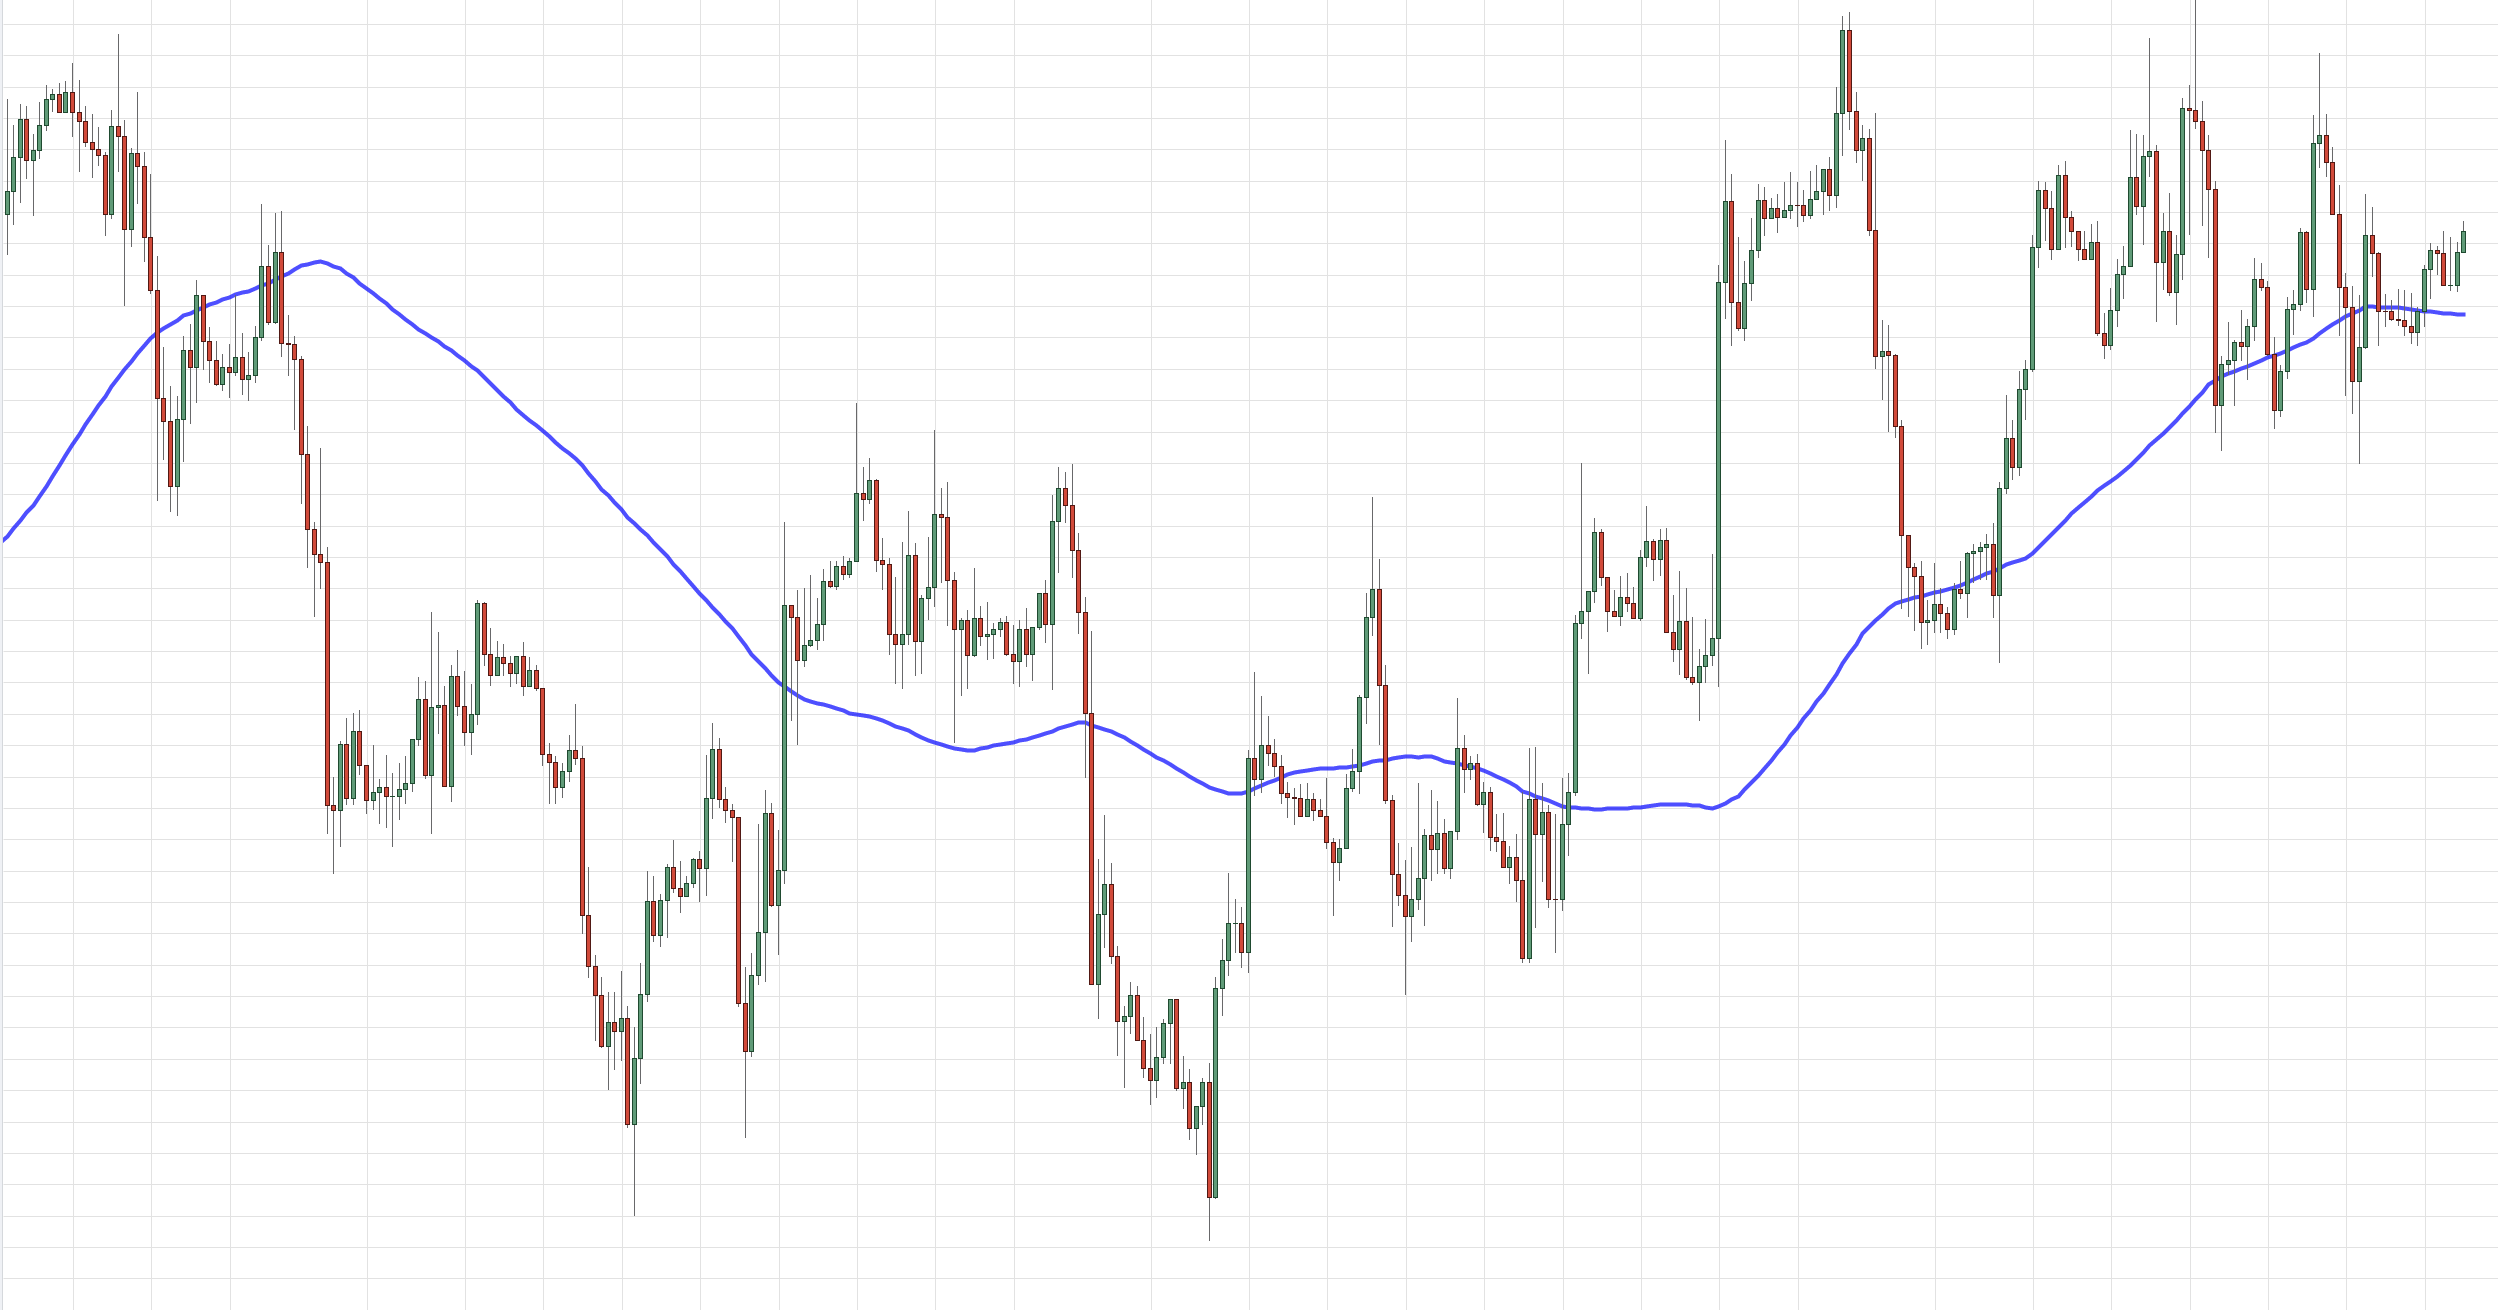
\includegraphics[width=0.8\textwidth]{img/fitting1.png}
% \label{figure:fitting1}
% \end{figure}

% \begin{figure}
% \caption{Fitting2}
% \centering
% 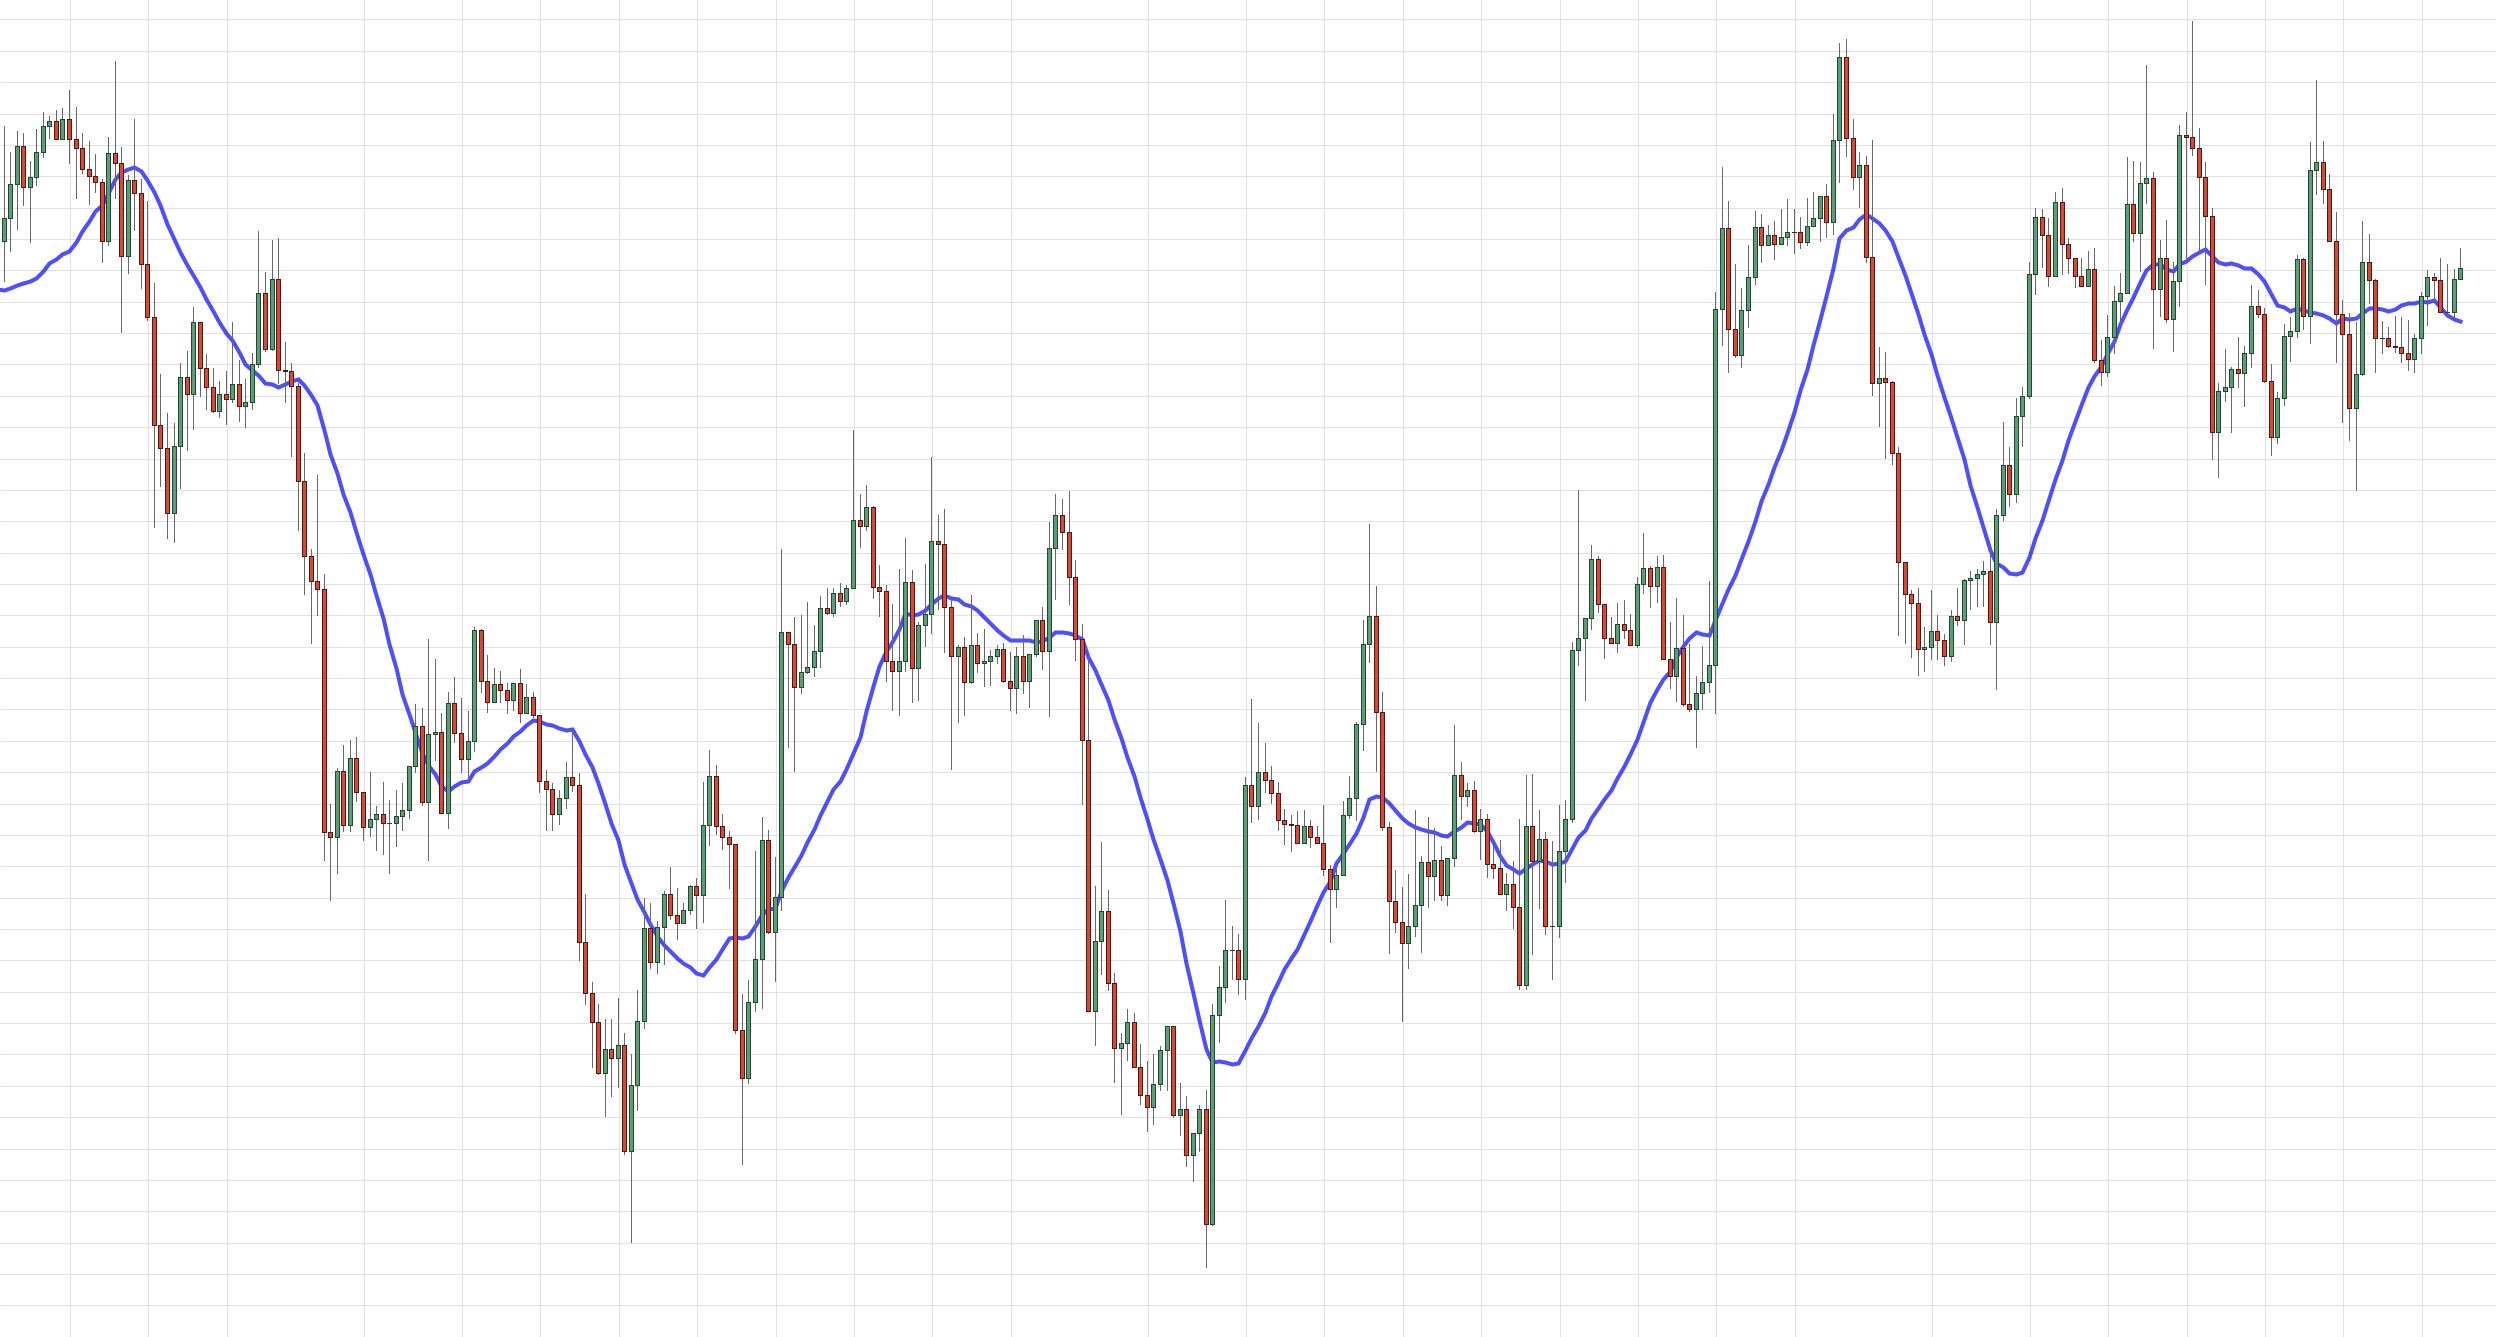
\includegraphics[width=0.8\textwidth]{img/fitting2.png}
% \label{figure:fitting2}
% \end{figure}

The agents in the prediction models are represented as objects with the following properties: agent's rules, which stores an intuitionistic fuzzy system; specializations, which stores the antecedents of the fuzzy system; and specialization thresholds, which stores the levels that need to be surpassed by a set of inputs in order to activate the agent.

Indeterminacy in an agent's fuzzy system is determined randomly and optimal values are found with the ILS method described in Subsection \ref{subsubsection:stochasticity}. In order to obtain intuitionistic fuzzy sets where (\ref{eq:intuitionistic-interval}) holds true, our implementation generates membership functions where the greatest possible grade of membership is $M$ and non-membership functions where the greatest possible grade of non-membership is $1 - M$. The mean and spread of the Gaussian membership functions are equal to the mean and spread of the Gaussian non-membership functions in all cases.

%\subsubsection{Collectives}
%\subsubsection{Observation}


\subsection{Details}
\label{subsection:details}

\subsubsection{Initialization}
\label{subsubsection:initialization}

The agents that are randomly generated for the ILS need to pass a test before they can be considered a candidate to be part of a predictive model. Considering a training data set, an agent's specialization functions are evaluated against the inputs set obtained from that training data set in order to generate a set of specializations, where each specialization is the equivalent of calculating the grade of membership associated to a set of inputs. 


After performing this step, all the specializations are summed to obtain a score $S$ that represents the intensity to which that agent reacts to that set of inputs. This score is defined by (\ref{equation:activation-score}), where $N$ represents the number of inputs, and $\mu(x_{i})$ represents each of the grades of membership associated to each input. The scores associated to each set of inputs are ordered in a descending manner, so the first elements are the scores that represent those sets of inputs that would fire an agent's consequents the most. The ordered scores list is also used to obtain the outputs that are associated to these ordered scores, so we can know what are the outputs that the agent \textit{should} evaluate to given those particular sets of inputs. The resulting set of outputs are used to determine if the agent is a suitable candidate; if most of the outputs associated to the highest scores have the same direction (negative or positive), then it is a suitable candidate. This mechanism ensures that the chosen agents are specialized in similar inputs that yield similar outputs. For our implementation, the highest scores have to be associated to outputs that share the same direction at least 66\% of the time. This value was chosen empirically after performing some preliminary tests, where different values greater than 50\%---as we want the majority of the outputs to share the same direction---were used. However, it is not statistically proven that this value will yield better results than other values.
% Why this arbitrary value? Is this a sensible/sensitive parameter?   - jj
% TODO 98: COMPLETE.

\begin{equation}
  \label{equation:activation-score}
  S =\sum_{i=1}^{N}{\mu(x_{i})}
\end{equation}

The optimization process for the predictive models loads configuration files as its first step, depending on the market that we want to use to obtain training and testing data sets. These configuration files set parameters for the proposed method, such as the train-test ratio and number of inputs, outputs and number of rules for the agents' fuzzy systems.

For our implementation of the proposed method we chose Common Lisp as our language, so we could use a software library for the creation of intuitionistic fuzzy systems that we implemented in the past \cite{Hernandez-Aguila2016} \cite{Hernandez-Aguila2017-2}. All the populations are compressed and stored in a PostgreSQL database, which enables us to resume the optimization of a model at any time. Storing the populations in a database also enables us to use populations of agents to be tested in other data sets, as well as to extract agents from certain populations to be used in other prediction models. The source code of our implementation can be found in the git repositories at this link: \url{https://bitbucket.org/overmind-group/workspace/projects/OT}.
% Opened an issue about the license; also, specify the concrete repository, not the general URL for all of them - JJ

The evaluation of the agents proved to be a computationally expensive task, as the system needs to evaluate hundreds of fuzzy systems per iteration in the optimization process. For this reason, we implemented a caching system where the output of an agent is stored in memory using a technique called \textit{memoization} \cite{johnson1995memoization} in a functional programming context. After \textit{memoizing} an agent, if that agent is required to be evaluated with exactly the same inputs as the ones used during the \textit{memoization} process, then we can assume that the output will be the same, and thus we can simply query for the output stored in memory. The caching system prevents our implementation from re-evaluating hundreds of fuzzy systems in the optimization process.

%\subsubsection{Input data}
%\label{subsubsection:input-data}

% I think this is a highlight, maybe going to intro  and abstract if this was
% tested - Mario
% TODO 37: COMPLETE. This was not tested, unfortunately. That's why I considered this
% only to be a technical peculiarity. Add a note if you still consider this to be
% a highlight worthy of being mentioned in the abstract and intro.

% The cahed of agents sounds interesting, maybe you should mentioned it
% if it reduced the training time - M
% TODO 38: COMPLETE. Added a paragraph explaining the caching system.

% We're using Common Lisp, an implementation of an intuitionistic fuzzy system
% We're saving our populations into a database, we can create branches, we can resume experiments.
% We're compressing our populations
% We're storing different metrics: MAPE, MASE, MAE, MSE, RMSE, Recall, Precision, F1-score, Accuracy, Revenue.
% MASE is not good if using activations because it depends on the next forecast.
% Storing popluations on a PostgreSQL database.
% Each individual agent can be evaluated to know what would be its trades given a data set.
% Agents are cached to improve computation performance.

% Activations are precomputed using if-membership. Indeterminacy is taken into account.
% Activations are reduced (summed) and we choose the greatest one (the one it is more fit to react to).
% We obtain what's the "wanted direction" (buy or sell) of that trade (the one with the greatest activation).
% Then I check the activations, ordered by how well they performed for this agent.
% The next N activations must be of the same direction than the first one. Discard agent otherwise.
% If all of them pass, then the activation threshold is the one at Nth position. So in theory each agent will trade N times, most of the time.

% Inderminacy is randomly determined from 0 to 1.
% The meta-heuristic will find heuristically if indeterminacy helps or not to activate or not.
% Already mentioned in proposed method I think: We take prices to be used as the means.

% An agent won't trade unless its inputs reach certain activation threshold.
% We check every trade to see if the agent trades or not.
% In case it passes: We use each input (price) to the fuzzy system, it fires a consequent, we do union, then if-coa, we obtain the mean of all these rules.
% Required activations (consecutive winning streak or we don't accept the agent).

% In draw optimization we're either removing an agent and checking if it's better or adding a new one and check if it's better.

% For each market we load configuration files that we determined heuristically, at random.
% We have a general file which indicates the percentage to use as test set, required activations, delta-gap, how many cores to use, what provider to use.
% Begin and end of datasets, extracts rates into global variable,
% We also have per-market config files that indicate how many data points to use as training data set, number of inputs, number of rules, inputs function.
% In experiments we provide the list of configurations per market.
% If no specific configuration file is found we use a predetermined configuration.

% We represent an agent as class that has the following slots: rules, activations, activation-threshold, consecutive-activations.

% We can use a population to be tested on any market, regardless of for what market that agent was trained for.
% List preprocessing functions:

% io-closes
% io-volumes
% io-highs
% io-lows
% io-high-heights
% io-low-heights
% io-candle-heights
% io-deltas
% io-full-heights
% io-fibos
% io-stochastic-oscillator
% io-sma
% io-awma
% io-ema
% io-macd
% io-macd-signal

%\subsubsection{Sub models}
%\label{subsubsection:sub-models}

\section{Experiments}
\label{section:experiments}

In order to determine the efficacy of the proposed method, we designed
experiments that involved data sets and performance metrics used in
the work by Munkhdalai et al. \cite{Munkhdalai2019}. In
\cite{Munkhdalai2019}, daily prices for the following Forex markets
are used: EUR/USD, USD/JPY, USD/CHF, GBP/USD, USD/CAD and AUD/USD. The last
year of prices are used as their data set, although they do not
provide the exact starting and ending dates. Their datasets are
partitioned into three parts: training, validation and test sets,
where the training set corresponds to 80\% of the data set, the
validation set corresponds to 10\% of the data set, and the test set
correspond to 10\% of the data set. The authors used a 5-fold time
series cross-validation method to obtain their performance metrics.

For our experiments, we decided to use random samples of 63 trading
days---which corresponds to a quarter of the trading days in a
year---for our data sets, which can be extracted from the last 5000
trading days (from August 28th 2004 to May 18th 2020). We did not use
the exactly the same data sets as Munkhdalai et al. because they do
not provide the starting and ending dates for their data sets, and
because a bigger data set---around 15 years of data, instead of 1 year
of data---provides a better challenge for avoiding accidental ``cherry
picking'' \cite{morse2010cherry} when choosing optimal hyperparameters
for the method. %
% why did you do this instead of the same thing as Munkhdalai - JJ
% TODO 100: COMPLETE.
These data sets
are split into two parts, a training data set which corresponds to
70\% of the data set, and a test data set which corresponds to 30\% of
the data set. As a consequence, a validation step was not involved in
our experiments. Regarding the performance metrics, we provide results
using MAE, in order to compare against the results presented
in \cite{Munkhdalai2019}. A total
of 30 experiments were performed for each forex market, and we provide
the means and standard deviations for each of our performance metrics
in Section \ref{section:results}.

In \cite{Munkhdalai2019}, the results of several predictive models are
provided. In order to obtain the hyper-parameters of the different
algorithms, random searching was used, with the exception of deep
learning neural networks (recurrent neural networks (RNN), long
short-term memory (LSTM) neural networks, and gated recurrent unit
(GRU) neural networks), where the learning rate was set at 0.001 using
the Adam optimizer \cite{kingma2014adam}, batch size at 64 instances
for each iteration, MSE as the loss function,and maximum number of
epochs at 3000 for the first fold, and then they used 300 epochs with
the first pre-trained model for the remaining folds. Regarding
multi-layer perceptrons (MLP), the authors used an input layer of 5 neurons
(for the prices of the last 5 days), a hidden layer of 16 neurons and
an output layer of 1 neuron (for the prediction of the next day's
price). In addition to neural network-based algorithms,
\cite{kingma2014adam} also provides results for models obtained by
random forest, AdaBoost, XGBoost and SVM
architectures.

Finding optimal values for the hyper-parameters of our method is a
challenge due to the high number of combinations that can lead to
favorable results. We decided to try to find arguments for these
parameters that allowed our method to generate models that yielded
results in the same order of magnitude as the results presented by its
competing methods. After some attempts, we arrived to the arguments
presented in Table \ref{agents-parameters}. In this table, %
% These are not parameters, but arguments - JJ
% Also, you need to present this as a challenge and show how you
% solved it - JJ
% Note: I checked the source code for that 6/9 trades part, and I noticed
% I removed it. Now I remember that it was something I was trying out but
% I didn't achieve noticeable differences in the algorithm performance. I'm
% removing that part (which is great, because it was utterly confusing, anyway).
$HH$ means ``high height'', and represents
the price difference between the high and the greater price between
close or open prices of a trading day; $LH$ means ``low height'', and
represents the price difference between the low and the lesser price
between close or open prices of a trading day; $CH$ means ``candle
height'' and represents the absolute price difference between the open
and close prices of a trading day; and the subscript following each of
the aforementioned abbreviations represents the number of past trading
days that were considered.

% Change table and figures' captions.
% TODO 39: COMPLETE. I'll do this for TODO #47.

\begin{table}[]
  \caption{Multi-agent systems parameters}
  \small
  \centering
  \begin{tabular}{cccc}
    \textbf{Market} & \textbf{\# of Inputs} & \textbf{\# of Rules} & \textbf{Inputs} \\
    \hline
    EUR/USD & 9 & 3 & $HH_3$, $LH_3$, $CH_3$ \\
    USD/JPY & 9 & 6 & $HH_3$, $LH_3$, $CH_3$ \\
    USD/CHF & 12 & 2 & $HH_4$, $LH_4$, $CH_4$ \\
    GBP/USD & 9 & 3 & $HH_3$, $LH_3$, $CH_3$ \\
    USD/CAD & 12 & 2 & $HH_4$, $LH_4$, $CH_4$ \\
    AUD/USD & 9 & 3 & $HH_3$, $LH_3$, $CH_3$ \\
    \hline
    \hline
    \# of iterations & \multicolumn{3}{c}{100} \\
    Loss function & \multicolumn{3}{c}{RMSE} \\
    \hline
  \end{tabular}
  \label{agents-parameters}
\end{table}

\section{Results}
\label{section:results}

Table \ref{table:comparison-mae} shows
subsets of the results presented by Munkhdalai et
al. \cite{Munkhdalai2019}, comparing them with the results of the
method presented in this paper. In the case of neural networks (RNN, GRU,
LSTM and MLP), the table shows the results obtained by Munkhdalai et
al., as well as the worst and best results that are not obtained
% confusing. Say how they are obtained, not how they are *not* obtaind
% - JJ
by
using the activation function proposed by Munkhdalai et al. In
addition to the neural network-based results, results for the
predictive models based on random forest, AdaBoost, XGBoost and
SVM are also provided. The purpose of this table
is to provide a comparison between the predictive models generated by
our proposed method and the predictive models generated by other
methods.

Our results can be found in the last rows of the table, and the best
result for each market is shown in bold. It must be noted that no
statistical testing was performed when comparing our method against
the ones provided by Munkhdalai et al.; the results in the table
have the purpose of showing the competitiveness of our method to some
extent, in terms of error, in order to justify further research to
improve our current method. Two results are presented for
our method: one where specialization functions (SF) are used to restrict agents
from certain trades, and another for agents not using specialization
functions to restrict their decisions. It is noteworthy that these
results cannot provide conclusive proof that one method is better than
another, as the testing datasets and methods are not the same. Table
\ref{table:full-results} provides again the means of our results, in
addition to their standard deviations, sample sizes and statistical
tests, where these statistical tests prove that the use of specialization
functions make our models perform better than those that do not use
specialization functions.

% But that was in the previous table
% also. What's the point? - JJ
% TODO: COMPLETE.

\begin{table*}[t]
  \caption{Comparison between our results and the ones obtained by Munkhdalai et al.}
  % Please explain that the bottom rows are compared in the table
  % below - JJ
  % Clarify also if the difference is significant with respect to
  % others - JJ
  % TODO: COMPLETE? I'm now mentioning in the paragraph above that the bottom rows represent
  %% our results, and that the table below shows additional data for statistical tests.
  %% I'm thinking that this clarifies that the difference between my two versions of the algorithm
  %% is significant.
  %% I was also thinking that maybe you wanted to add an explanation to the caption of this table.
  %% Can you give me a more detailed explanation of your request? (in case it's not solved already by my changes).
  \scriptsize
  \centering
  \begin{tabular*}{0.9\textwidth}{c @{\extracolsep{\fill}} ccccccc}
    \hline
    \textbf{Model} & \textbf{Specialization function} & \textbf{EUR/USD} & \textbf{USD/JPY} & \textbf{USD/CHF} & \textbf{GBP/USD} & \textbf{USD/CAD} & \textbf{AUD/USD} \\
    \hline

          & Sigmoid & 0.0060 & 5.4000 & 0.0081 & 0.0126 & 0.0060 & 0.0079 \\
    RNN   & Swish & 0.0044 & 0.4925 & 0.0042 & 0.0074 & 0.0068 & 0.0043 \\
          & Munkhdalai et al. & 0.0043 & 0.4479 & 0.0037 & 0.0083 & 0.0047 & 0.0034 \\
    \hline
          & Cosine & 0.0098 & 2.0191 & 0.0130 & 0.0396 & 0.0106 & 0.0162 \\
    GRU   & Linear & 0.0044 & 0.4475 & 0.0041 & 0.0083 & 0.0052 & 0.0041 \\
          & Munkhdalai et al. & 0.0044 & 0.5327 & 0.0039 & 0.0062 & 0.0046 & 0.0071 \\
    \hline
          & ReLU & 0.0053 & 1.4920 & 0.0054 & 0.0101 & 0.0058 & 0.0046 \\
    LSTM  & Swish & 0.0045 & 0.5243 & 0.0049 & 0.0065 & 0.0063 & 0.0054 \\
          & Munkhdalai et al. & 0.0046 & 0.5200 & 0.0060 & 0.0069 & 0.0061 & 0.0044 \\
    \hline

          & ReLU & 0.0049 & 0.7499 & 0.0058 & 0.0150 & 0.0052 & 0.0038 \\
    MLP   & Swish & 0.0043 & 0.7351 & 0.0039 & 0.0073 & 0.0055 & 0.0042 \\
          & Munkhdalai et al. & 0.0047 & 0.6114 & 0.0059 & 0.0066 & 0.0049 & 0.0041 \\
          

    \hline

    \multicolumn{2}{l}{Random forest} & 0.0053 & 0.5209 & 0.0061 & 0.0156 & 0.0059 & 0.0044 \\
    \multicolumn{2}{l}{AdaBoost} & 0.0059 & 0.6440 & 0.0103 & 0.0158 & 0.0063 & 0.0066 \\
    \multicolumn{2}{l}{XGBoost} & 0.0059 & 0.4958 & 0.0048 & 0.0156 & 0.0064 & 0.0045 \\
    \multicolumn{2}{l}{SVM} & 0.0304 & 0.4718 & 0.0376 & 0.0294 & 0.0099 & 0.0176 \\

    \hline
    \hline
    
    \multicolumn{2}{l}{Ours without SF}        & 0.0050          & 0.4903          & 0.0041          & 0.0073          & 0.0050          & 0.0048 \\
    \multicolumn{2}{l}{Ours with SF}           & \textbf{0.0033} & \textbf{0.1810} & \textbf{0.0019} & \textbf{0.0038} & \textbf{0.0033} & \textbf{0.0027} \\
    \hline

  \end{tabular*}
  \label{table:comparison-mae}
\end{table*}

% Tables \ref{table:full-results-no-activations}
% \ref{table:full-results-activations}
% and \label{table:full-results-weights} provide results involving
% different versions of our proposed method. Table
% \ref{table:full-results-no-activations} shows results for a
% multi-agent system where agents have no activation functions---which
% means that agents respond to any set of inputs. Table
% \ref{table:full-results-activations} shows results for a
% multi-agent system where agents have activation functions, exactly as
% described in Section \ref{section:proposed-method}. Lastly, Table
% \ref{table:full-results-activations} shows results for a modified
% version of our proposed method, where the output of an agent's
% activation function is used a weight that is multipiled by that
% agent's output, instead of using the activation function as a
% threshold, as in the proposed method.

\begin{table*}[t]
  \caption{Results of our method with and without specialization functions to restrict their actions}
  \scriptsize
  \centering
  \begin{tabular*}{0.9\textwidth}{c @{\extracolsep{\fill}} ccccccc}
    \hline
    \multicolumn{2}{c}{\textbf{Metric}} & \textbf{EUR/USD} & \textbf{USD/JPY} & \textbf{USD/CHF} & \textbf{GBP/USD} & \textbf{USD/CAD} & \textbf{AUD/USD} \\
    \hline
                                        & $n$ & 60 & 60 & 60 & 60 & 60 & 60 \\
                                        & $n_{SF}$ & 50 & 51 & 56 & 51 & 50 & 44 \\
    \hline
    \multirow{3}{*}{MAE} & Mean & 5.03\e{-03} & 4.90\e{-01} & 4.13\e{-03} & 7.34\e{-03} & 5.05\e{-03} & 4.83\e{-03} \\
                                        & Std dev & 2.79\e{-03} & 2.20\e{-01} & 1.94\e{-03} & 4.01\e{-03} & 2.24\e{-03} & 2.12\e{-03} \\
    \multirow{3}{*}{MAE\textsubscript{SF}} & Mean & 3.27\e{-03} & 1.81\e{-01} & 1.95\e{-03} & 3.80\e{-03} & 3.32\e{-03} & 2.74\e{-03} \\
                                        & Std dev & 3.81\e{-03} & 1.31\e{-01} & 1.53\e{-03} & 3.12\e{-03} & 1.94\e{-03} & 2.25\e{-03} \\
    \hline
    \hline
                                        & $t-value$ & -2.71555 & -9.13914 & -6.74278 & -5.2259 & -4.3400 & -4.7952 \\
                                        & Conclusion & Reject $H_0$ & Reject $H_0$ & Reject $H_0$ & Reject $H_0$ & Reject $H_0$ & Reject $H_0$ \\
    \hline
    \hline
  \end{tabular*}
  \label{table:full-results}
\end{table*}

\begin{table}[]
  \caption{Parameters used for the hypothesis tests}
  \small
  \centering
  \begin{tabular}{lc}
    \textbf{Parameter} & \textbf{Value} \\
    \hline
    Confidence interval & 95\% \\
    $H_a$ & $\mu_1 < \mu_2$ \\
    $H_0$ & $\mu_1 \geq \mu_2$ \\
    Critical t & -1.9958 \\
  \end{tabular}
  \label{table:parameters-tests}
\end{table}

\section{Conclusion}
\label{section:conclusion}

% Check that we mention all of these contributions in here:
% i) our method describes a novel architecture that mixes MAS and fuzzy systems for
% the creation of predictive models;
% x ii) the activation functions found in the agents' fuzzy systems help to decrease the error between
% predicted and real market prices;
% iii) the results from the experiments indicate us that the models generated by our method are
% competitive against models generated by deep learning, random forest,
% AdaBoost, XGBoost and support-vector machines;
% iv) our method describes a simple and effective method for the tuning of parameters for MAS.
% TODO 41: COMPLETE.

Financial markets are examples of complex systems, which is why they
can be better represented using agent-based models. The advantage of these models, which are capable of simulating the
simultaneous operations and interactions of multiple agents, is that they can
re-create and predict the behavior resulting from the complex phenomena of
emergence. These models have the additional advantage of being interpretable and
can give us additional knowledge about the dynamics of the market.

In this work, we proposed a MAS that models agents' knowledge as
intuitionistic fuzzy inference systems, along with specialization
functions that allow agents to become specialized for trading
particular market conditions. The MAS was adjusted to obtain a forex
market predictive model by using our proposed ILS to optimize the
models' parameters.

To evaluate our model's predictive performance, we compare it against
models generated by RNN, LSTM, GRU, MLP, random forest, AdaBoost,
XGBoost, and SVM. The results lead us to conclude that our method
proves to be competitive for predicting forex markets, as shown in
Table \ref{table:comparison-mae}, where our method performed the best
for every forex market, if our models use specialization functions. We
decided to use MAE as our performance measurement as MAE works well
when the error distribution is not Gaussian---which is the case for
our method, as agents not always decide to take trades---, in contrast
to other metrics, such as RMSE \cite{chai2014root}, and because it has
been reported to be a good metric for measuring the performance of
predictive models \cite{willmott2005advantages}
\cite{willmott2009ambiguities}.


Furthermore, according to the experiments, the use of specialization
functions decreases the predictive error. This demonstrates that using
them to create agents that are specialized at
particular market conditions help to increase the generated models'
efficacy.


%Table \ref{table:full-results} provides a
%more complete overview of our results, as it shows the means and
%standard deviations of our errors, along with hypothesis testings that
%prove that, for the datasets used, our method performs better with the
%use of activation functions.
% This was explained in the results section, it does not need to be repeated here.

% Can this be generalized? - JJ Done - M

% Conclusions shouldn't just enunciate results (that should be done above), 
% it should try and explain why they happen. Is there something in that 
% specific dataset that makes it work better without AF? - JJ
% Agree, I commented these repetitions - M

% Please see the comment at the bottom - JJ
% You would need to generalize this, so that someone decides, 
% on the basis of this characterization, 
% whether your method or Munkdalai's is better - JJ

% Please summarize. I'm kind of lost. You seem to be drawing 
% conclusions on how to measure performance, but there should 
% be an objective way of doing so: ROI? You're kind of saying our method is good,
% but only if we measure it that way. If we do it in some other way,
% well, not so good. What's the deal then? Is this paper about evaluation of metrics?
% You need to give conclusive results in the conclusion. 
% We think this metric is better, so our method is better and that's that. - JJ

% We settled for just reporting MAE and RMSE - M

%Finally, it must be noted that the results shown in
%Table \ref{table:comparison-mae} have the
%purpose of demonstrating the competitiveness of our method for the
%creation of predictive models. Concluding that our method is better
%than the others shown in that table would be na\"ive, as the datasets
%used in our experiments and the methods used for testing the
%performance of the models differ to those used by Munkhdalai in
%\cite{Munkhdalai2019}. 


% Explain more this advantage. 
In addition to the low predictive errors obtained, it should be noted
that our method has the advantage of being more interpretable than the
method proposed by Munkhdalai et al. The agents in our predictive models can
be displayed as membership functions being activated by inputs,
along with their consequents being alpha-cut, aggregated and
deffuzified to a final output value. The user can easily examine the
rules that the agents are following and thus have a clear picture of
how the agents react to the prices. For example, consider the
following fuzzy rules:

\begin{enumerate}
	\item if RSI(x) is LOW, then BUY is HIGH
	\item if RSI(x) is MEDIUM, then BUY is MEDIUM
	\item if RSI(x) is HIGH, then BUY is LOW
\end{enumerate}

If an agent is performing very well during the current market
conditions, we can then assume that there is a relationship between
the technical indicator $RSI$ and upward directional movements. After
examining multiple agents, we can draw more complex conclusions about
a market.

% This is not proved, however. You need to show the method and how to
% interpret it. You have evaluated your method and compared it 
% in a number of ways, and they said that the result is not conclusive.
% So why did you compare it? Shouldn't you compare it in tasks that are similar? - JJ

% I agree - Mario 

As can be concluded, choosing the correct technical indicators or any
other functions that preprocess the agents' inputs is crucial for
generating knowledge that can be interpreted by the user. Furthermore,
the selection of these functions, along with every other value for the
parameters of our method is equally as important. Currently, our
implementation does not have a mechanism for the selection of optimal
values for these parameters. A user of our method would need to search
by trial and error for values that yield desirable results according
to the nature of the problem they want to model.

\section{Future Work}
\label{section:future-work}

The experiments presented in this work demonstrate that better
methodologies need to be used in order to provide conclusive proof
that the use of specialization functions in the agents' fuzzy systems is
beneficial for the creation of predictive models. Additionally, we can
test our specialization functions in other methods, such as neural
networks. Furthermore, we could design experiments that demonstrate
which version of our method helps real traders make better decisions.

The proposed method was tested using a subset of all the forex markets
currently available. More experiments could be performed where
additional forex markets are tested. Moreover, our method should be
tested with financial markets of different natures, such as stocks,
bonds, commodities and metals.

An advantage of fuzzy systems over other modelling techniques is that
fuzzy systems are interpretable. Natural language processing
techniques that use the fuzzy systems as inputs could be used to
provide texts that describe the conditions of a market, as perceived
by the agents in the MAS.

Our implementation should be adapted to perform in a distributed
manner, where agents are evaluated in parallel in different CPU cores
or even different physical machines. A distributed architecture will
help achieve results faster, which will allow us to test different
approaches for the creation of predictive models using our method.

Finally, the ILS method used for optimization in the proposed method should be
benchmarked against other optimization techniques, such as genetic
algorithms or particle swarm optimization. Finding better optimization
algorithms for our method can help us achieve better results, and probably faster. It is
also probable that lower errors could be achieved, as we do not know
if our current optimization method is exploring a wide enough search space.

\section*{Acknowledgment}
This paper has been supported in part by project DeepBio (TIN2017-85727-C4-2-P).

\begin{IEEEbiography}[{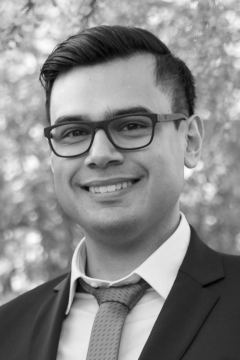
\includegraphics[width=1in,height=1.25in,clip,keepaspectratio]{img/amaury-1by1half-in.png}}]{Amaury
  Hernandez-Aguila}

  Amaury Hernandez-Aguila received the Ph.D degree in Computer Science and the
  M.Sc. degree in Computer Science from the Tijuana Institute of Technology,
  Mexico, in 2014 and 2019, respectively. He is currently participating in a
  post-doctoral program in Tijuana Institute of Technology, researching how
  multi-agent systems and fuzzy logic can be used for the prediction of
  financial markets. In addition to research, he is working for a company based
  in Shanghai, China, where he is the lead designer and developer of a
  blockchain-based programming language called CX.

\end{IEEEbiography}

\begin{IEEEbiography}[{
\includegraphics[width=1in,height=1.25in,clip,keepaspectratio]{img/Garcia.jpg}}]{Mario García Valdez} 
  Dr. García-Valdez is a full-time research professor at the Tijuana
  Institute of Technology. He's interested in the personalization of
  interactive systems, voluntary computing, parallel evolutionary
  computation, interactive evolutionary computation.
\end{IEEEbiography}

\begin{IEEEbiography}[{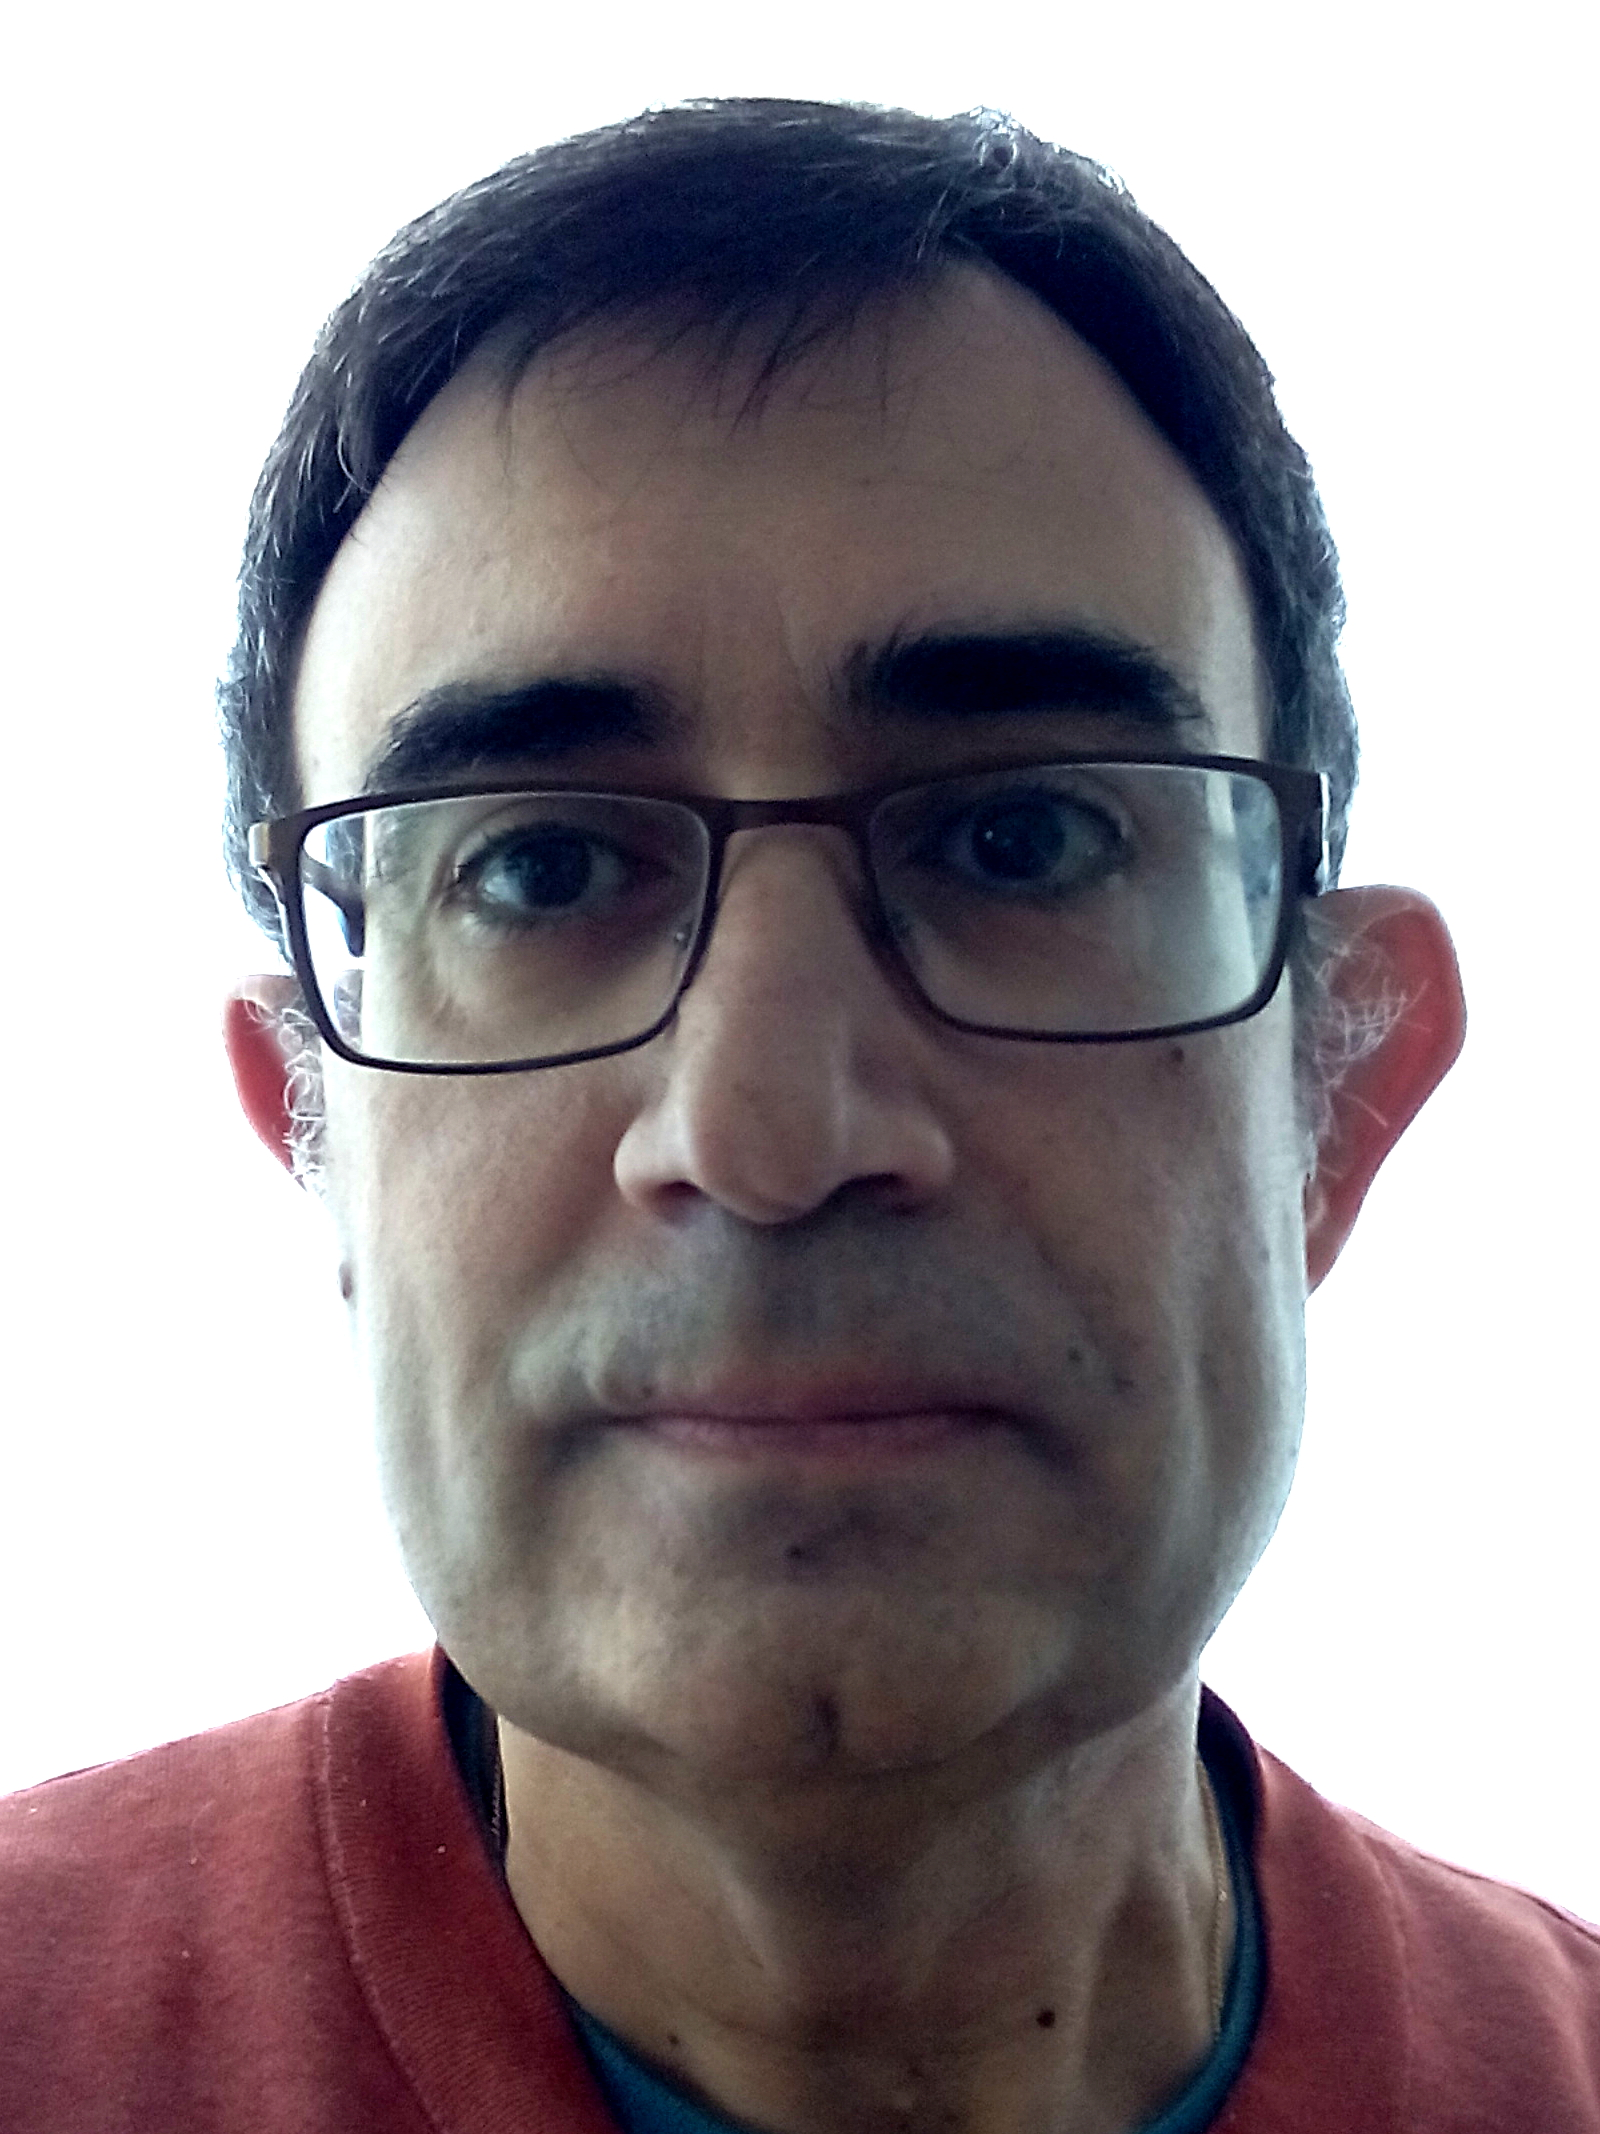
\includegraphics[width=1in,height=1.25in,clip,keepaspectratio]{img/jj-2016-10.jpg}}]{JJ Merelo Guervós} 
  JJ Merelo is professor at the university of Granada, where he obtained a
  degree in Theoretical Physics and a PhD in Physics in 1994. He's mainly
  interested in evolutionary algorithms, open source software and complex
  systems.
  
\end{IEEEbiography}

\begin{IEEEbiography}[{
\includegraphics[width=1in,height=1.25in,clip,keepaspectratio]{img/Puga.jpg}}]{Manuel
Castañón Puga} Manuel Castañón-Puga is Professor at Autonomous University of
Baja California. He obtained a PhD on Computer Sciences from Autonomous
University of Baja California in México, and a Masters on Computer Sciences and
Bachelor in Engineering at Tijuana Technology Institute, in his native Tijuana,
México. His research of modeling and simulation, agent-base simulation,
hybrid-intelligent agents and multi-agent systems explores the way in which
software agents could be used to describe multidimensional environments,
innovation, evolution and adaptation in complex adaptive systems. Dr.
Castañón-Puga collaborates with multidisciplinary researchers and scientists to
create multidimensional computer simulations of societies, political ideologies,
trading economies and urban landscapes. His research also intends to incorporate
the ideas of complexity into the mainstream of engineering and in particular to
its instruction at the undergraduate level. \end{IEEEbiography}


\begin{IEEEbiography}[{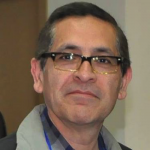
\includegraphics[width=1in,height=1.25in,clip,keepaspectratio]{img/Castillo.png}}]{Oscar
Castillo López} Oscar Castillo holds the Doctor in Science degree (Doctor
Habilitatus) in Computer Science from the Polish Academy of Sciences.
He is a Professor of Computer Science in the Graduate Division, Tijuana
Institute of Technology, Tijuana, Mexico. In addition, he is serving as Research
Director of Computer Science and head of the research group on Hybrid Fuzzy
Intelligent Systems. Currently, he is President of HAFSA (Hispanic American
Fuzzy Systems Association) and Past President of IFSA (International Fuzzy
Systems Association). Prof. Castillo is also Chair of the Mexican Chapter of the
Computational Intelligence Society (IEEE). He also belongs to the Technical
Committee on Fuzzy Systems of IEEE and to the Task Force on “Extensions to
Type-1 Fuzzy Systems”. He is currently Associate Editor of the Information
Sciences Journal, Applied Soft Computing Journal, Journal of Engineering
Applications on Artificial Intelligence, Granular Computing Journal and the
International Journal of Fuzzy Systems. Finally, he recently received the Recognition as
Highly Cited Researcher in 2017 and 2018 by Clarivate Analytics and Web of
Science \end{IEEEbiography}

\bibliography{bibliography}
\bibliographystyle{IEEEtran}

\EOD

\end{document}